% \documentclass[aspectratio=169,notes]{beamer}
\documentclass[aspectratio=169]{beamer}
\usetheme[faculty=phil]{fibeamer}
\usepackage{polyglossia}
\setmainlanguage{english} %% main locale instead of `english`, you
%% can typeset the presentation in either Czech or Slovak,
%% respectively.
\setotherlanguages{russian} %% The additional keys allow
%%
%%   \begin{otherlanguage}{czech}   ... \end{otherlanguage}
%%   \begin{otherlanguage}{slovak}  ... \end{otherlanguage}
%%
%% These macros specify information about the presentation
\title[IME]{Introduction to Mechanical Engineering, Lecture 5} %% that will be typeset on the
\subtitle{Connections:
\\ Detachable (Threaded, Keyed, ...) \\   
Permanent (Riveting, Welding, ...)} %% title page.
\author{Oleg Bulichev}
%% These additional packages are used within the document:
\usepackage{ragged2e}  % `\justifying` text
\usepackage{booktabs}  % Tables
\usepackage{tabularx}
\usepackage{tikz}      % Diagrams
\usetikzlibrary{calc, shapes, backgrounds}
\usetikzlibrary{decorations.pathreplacing,calligraphy,calc,graphs}
\usepackage{amsmath, amssymb}
\usepackage{url}       % `\url`s
\usepackage{listings}  % Code listings
% \usepackage{subfigure}
\usepackage{floatrow}
\usepackage{subcaption}
\usepackage{mathtools}
\usepackage{todonotes}
\usepackage{fontspec}
\usepackage{multicol}
\usepackage{pdfpages}
\usepackage{wrapfig}
\usepackage{animate}
\usepackage{booktabs}
\usepackage{multirow}
% \usepackage{graphicx}
\usepackage{colortbl}

\graphicspath{{resources/}}
\frenchspacing

\setbeamertemplate{caption}[numbered]
\usetikzlibrary{graphs}

% \usepackage[backend=biber,style=ieee,autocite=footnote]{biblatex}
% \addbibresource{biblio.bib}
% \DefineBibliographyStrings{english}{%
%   bibliography = {References},}

\newcommand{\oleg}[2][] {\todo[color=red, #1] {OLEG:\\ #2}}
\newcommand{\fbckg}[1]{\usebackgroundtemplate{\includegraphics[width=\paperwidth]{#1}}}%frame background

\usepackage[framemethod=TikZ]{mdframed}
\newcommand{\dbox}[1]{
\begin{mdframed}[roundcorner=3pt, backgroundcolor=yellow, linewidth=0]
\vspace{1mm}
{#1}
\vspace{1mm}
\end{mdframed}
}

\begin{document}
\setlength{\abovedisplayskip}{0pt}
\setlength{\belowdisplayskip}{0pt}
\setlength{\abovedisplayshortskip}{0pt}
\setlength{\belowdisplayshortskip}{0pt}

\fbckg{fibeamer/figs/title_page.png}
\frame[c]{\setcounter{framenumber}{0}
    \usebeamerfont{title}%
    \usebeamercolor[fg]{title}%
    \begin{minipage}[b][6.5\baselineskip][b]{\textwidth}%
        \textcolor{black}{\raggedright\inserttitle}
    \end{minipage}
    % \vskip-1.5\baselineskip

    \usebeamerfont{subtitle}%
    \usebeamercolor[fg]{framesubtitle}%
    \begin{minipage}[b][3\baselineskip][b]{\textwidth}
        \raggedright%
        \insertsubtitle%
    \end{minipage}
    \vskip.25\baselineskip
}
%   \frame[c]{\maketitle}

\fbckg{fibeamer/figs/common.png}

\note{\scriptsize \begin{itemize}
        \item \
    \end{itemize}}

\begin{frame}[t]{Connections}
    \framesubtitle{Classification}
    \vspace{-0.7cm}
    \begin{figure}[H]
        \begin{subfigure}{0.48\textwidth}
            \centering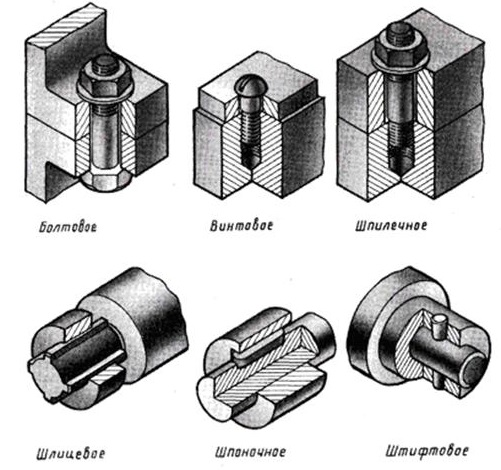
\includegraphics[height=5.5cm,width=1\textwidth,keepaspectratio]{detach.jpg}
            \caption*{Detachable (Разъемные)}
            \label{fig:detach.jpg}
        \end{subfigure}
        \begin{subfigure}{0.48\textwidth}
            \centering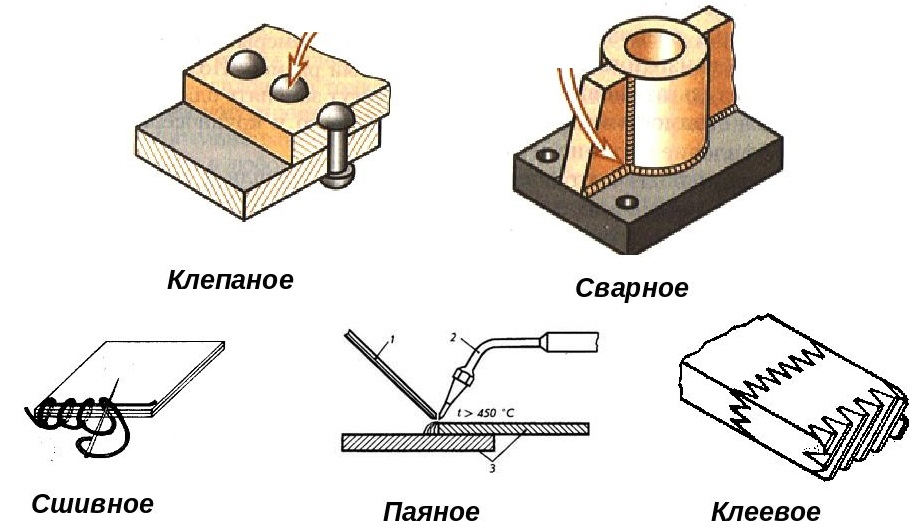
\includegraphics[height=5.5cm,width=1\textwidth,keepaspectratio]{fixed.jpg}
            \caption*{Permanent (Неразъемные)}
            \label{fig:fixed.jpg}
        \end{subfigure}
    \end{figure}
\end{frame}

\begin{frame}[t]{Keyed (Шпоночное) and Spline (Шлицевое)}
    \framesubtitle{}
    \begin{columns}[T,onlytextwidth]
        \begin{column}{0.49\textwidth}
            Using keyed connection, you can attach, gears, pulleys, and cams on shafts to obtain machinery.
        \end{column}
        \begin{column}{0.49\textwidth}
            \begin{figure}[H]
                \centering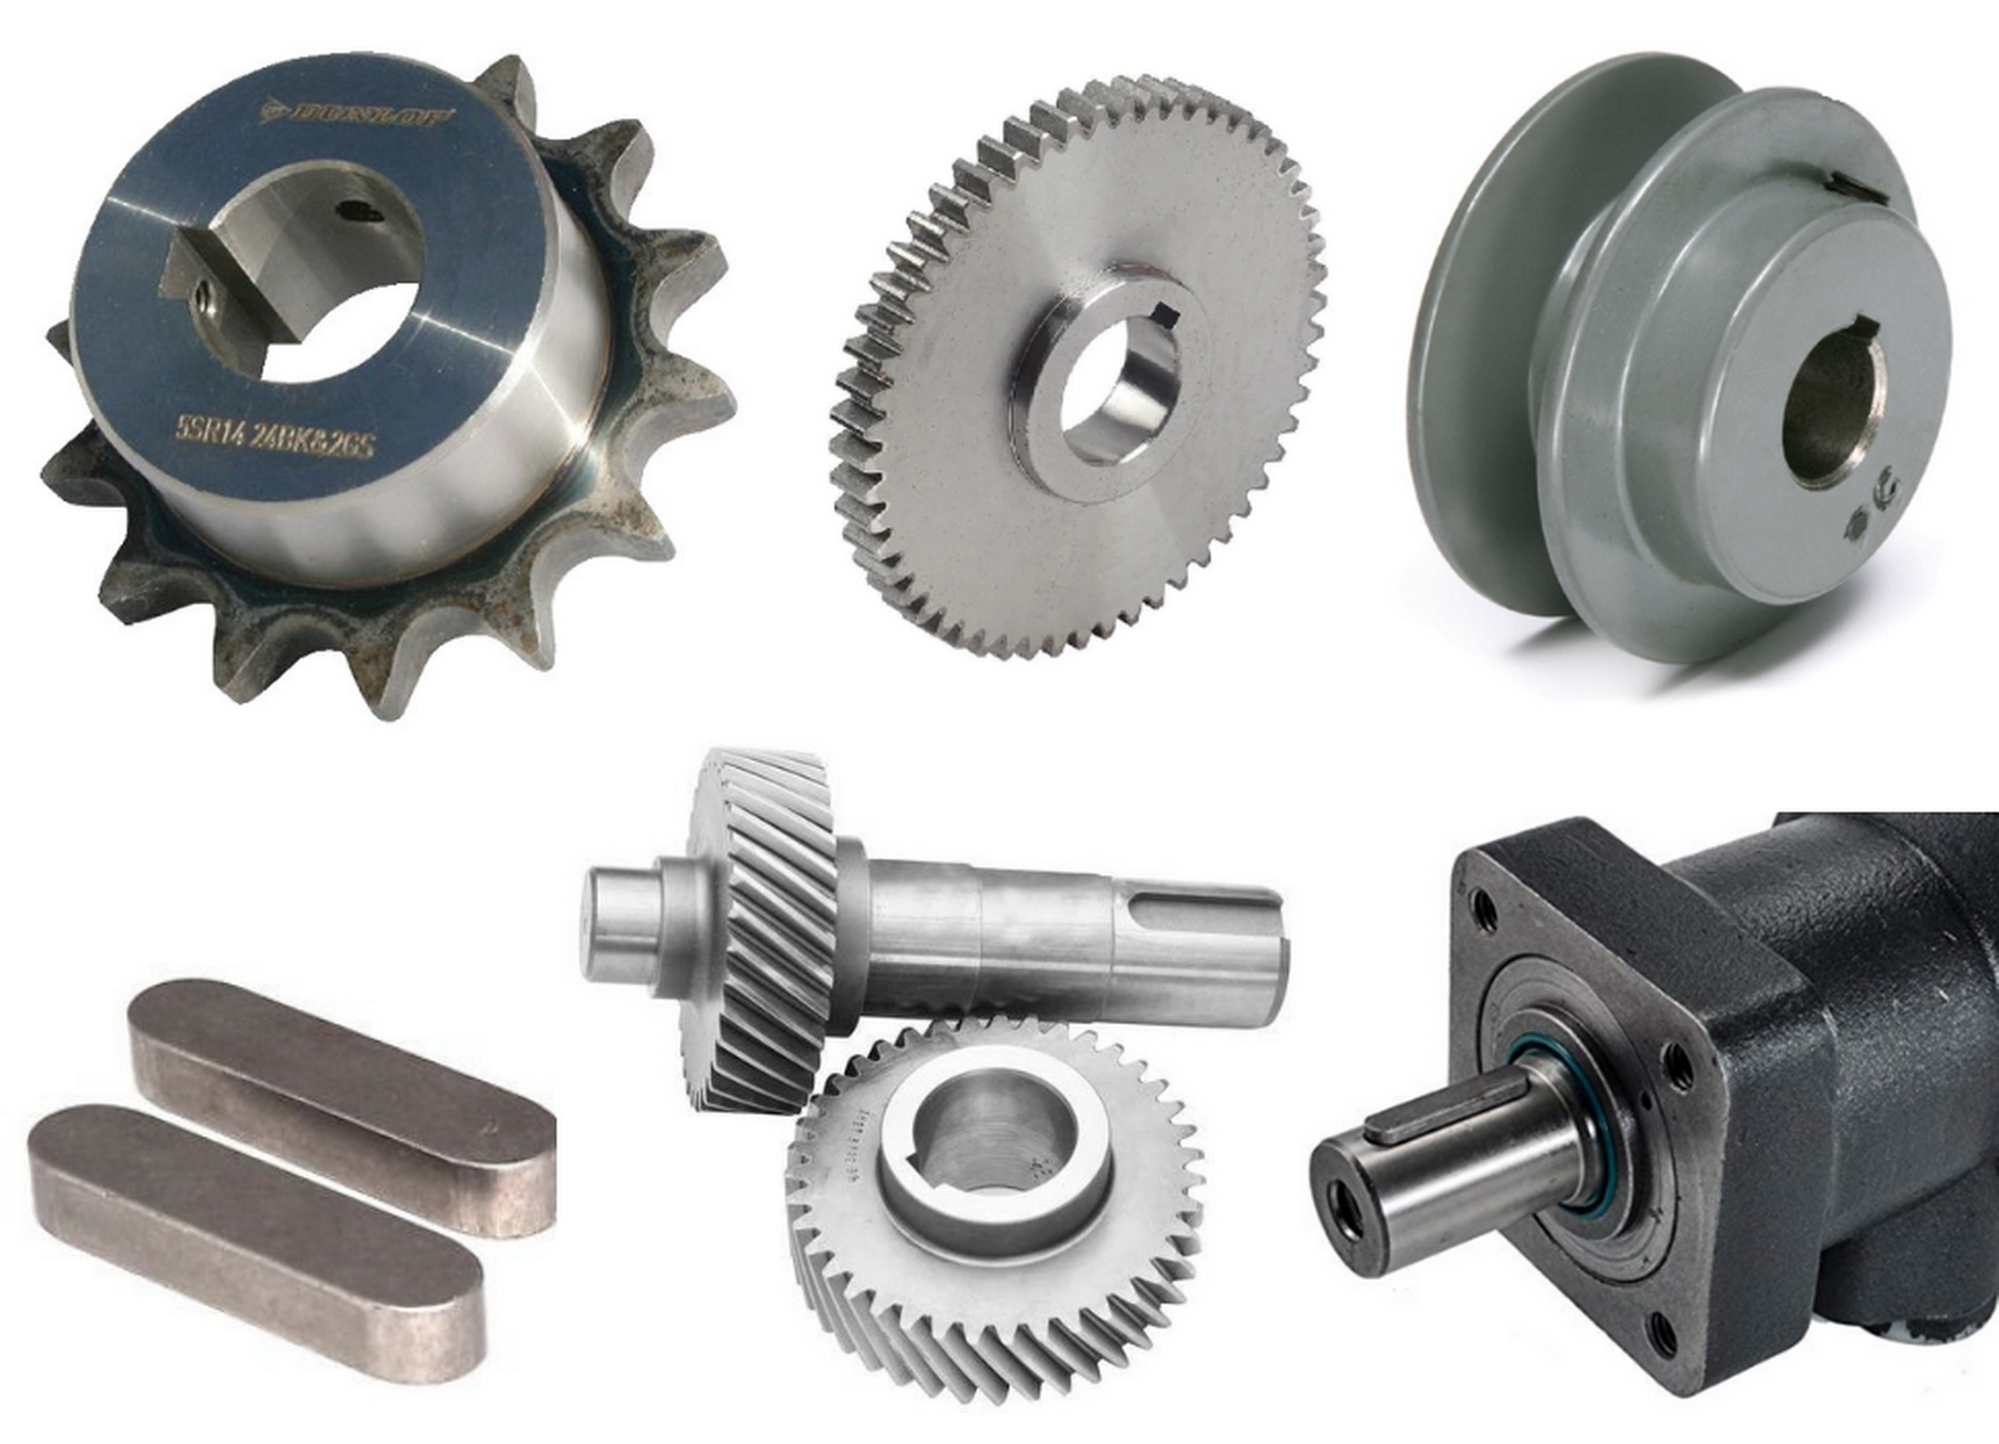
\includegraphics[height=5cm,width=1\textwidth,keepaspectratio]{find_key.png}
                \label{fig:find_key.png}
            \end{figure}
        \end{column}
    \end{columns}
\end{frame}

\begin{frame}[t]{Types of keys}
    \framesubtitle{Video}
    \vspace{-0.6cm}
    \begin{figure}[H]
        \href{https://youtu.be/F3c6GPAFZMI}{
            \centering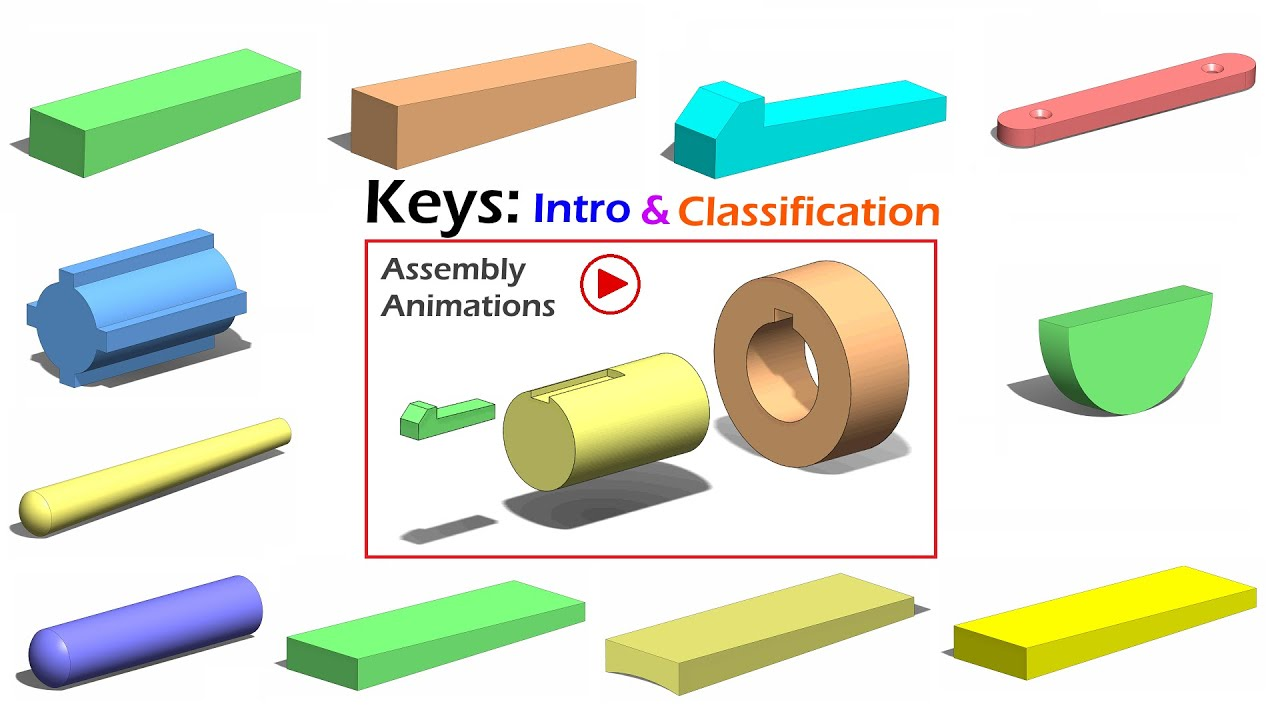
\includegraphics[height=6cm,width=1\textwidth,keepaspectratio]{keyed_video.jpg}}
        \label{fig:keyed_video.jpg}
    \end{figure}
\end{frame}

\begin{frame}[t]{Types of keys}
    \framesubtitle{}
    \vspace{-0.6cm}
    \begin{figure}[H]
        \centering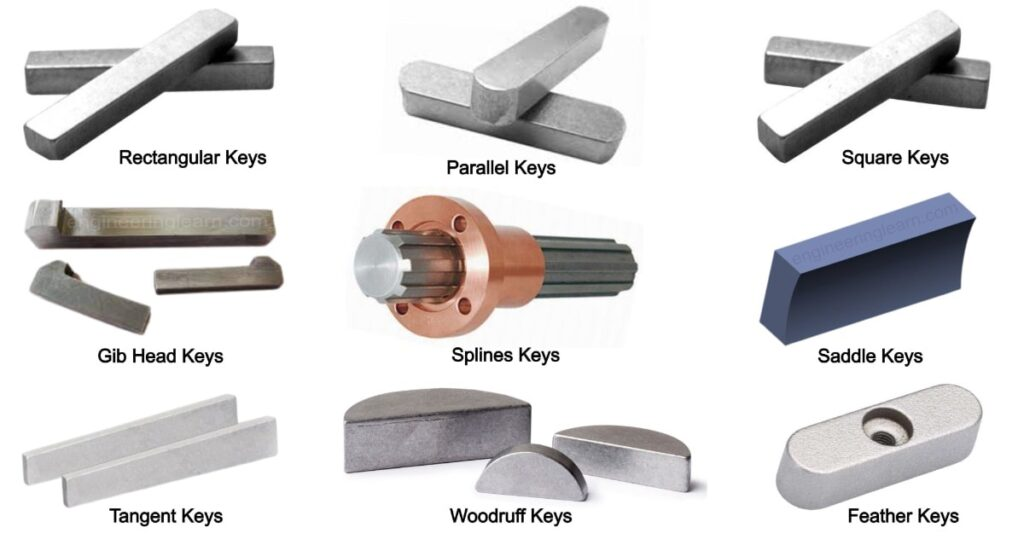
\includegraphics[height=6cm,width=1\textwidth,keepaspectratio]{types_of_keys.jpg}
        \label{fig:types_of_keys.jpg}
    \end{figure}
\end{frame}

\begin{frame}[t]{Keys and Splines (rus)}
    \framesubtitle{Video}
    \vspace{-0.6cm}
    \begin{figure}[H]
        \href{https://youtu.be/-bktOSXtLB8}{
            \centering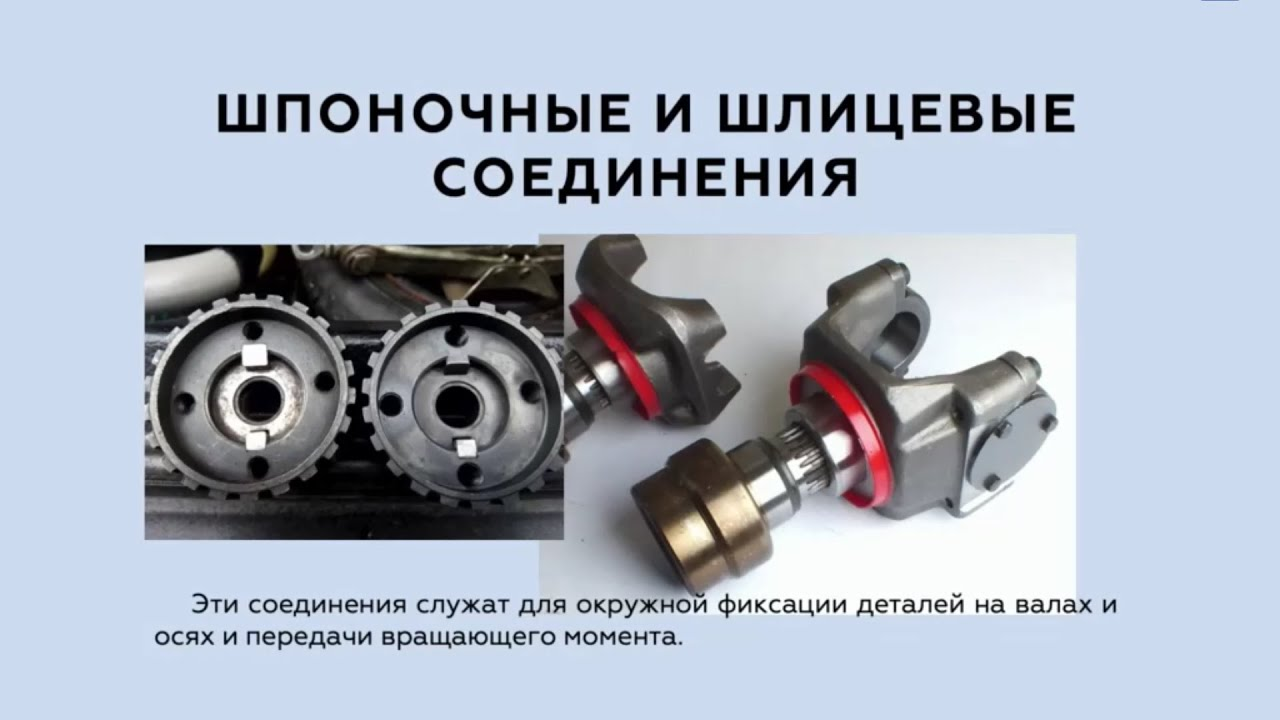
\includegraphics[height=6cm,width=1\textwidth,keepaspectratio]{key_rus_video.jpg}}
        \label{fig:key_rus_video.jpg}
    \end{figure}
\end{frame}

\begin{frame}[t]{Keyed connection}
    \framesubtitle{Reference material}
    \begin{itemize}
        \item \href{https://mechanicalland.com/shaft-keys/}{Shaft Keys and Keyways; Design, Explanation Applications}
    \end{itemize}
\end{frame}


\begin{frame}[t]{Pin (Штифтовое)}
    \framesubtitle{}
    \begin{columns}[T,onlytextwidth]
        \begin{column}{0.49\textwidth}
            It is a fastening element in the form of a cylindrical or tapered rod designed for a fixed connection. 
            
            The pin is inserted tightly into the hole that runs through both parts, preventing their mutual displacement.
        \end{column}
        \begin{column}{0.49\textwidth}
            \begin{figure}[H]
                \centering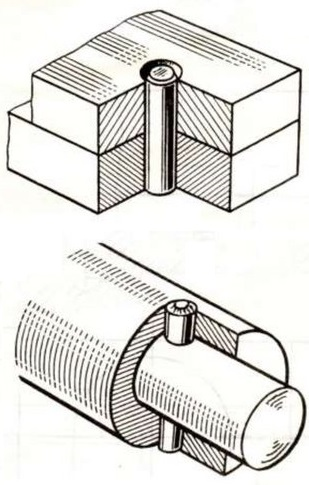
\includegraphics[height=5cm,width=1\textwidth,keepaspectratio]{stift.jpg}
                \label{fig:stift.jpg}
            \end{figure}
        \end{column}
    \end{columns}
\end{frame}

\begin{frame}[t]{Types of pin connections}
    \framesubtitle{}
    \vspace{-0.6cm}
    \begin{columns}[T,onlytextwidth]
        \begin{column}{0.69\textwidth}
            \begin{figure}[H]
                \begin{subfigure}{0.49\textwidth}
                    \centering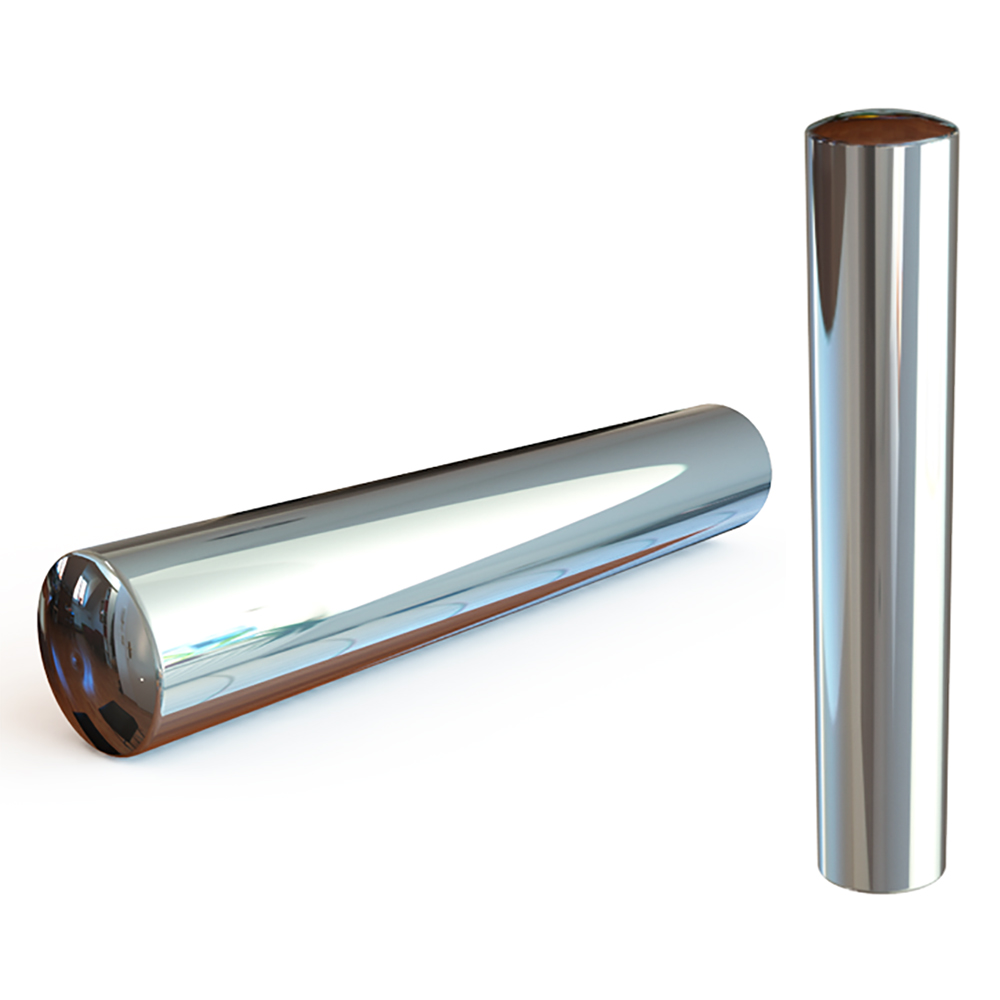
\includegraphics[height=3cm,width=1\textwidth,keepaspectratio]{pin_1.png}
                    % \caption{capture1}
                    \label{fig:pin_1.png}
                \end{subfigure}
                \begin{subfigure}{0.49\textwidth}
                    \centering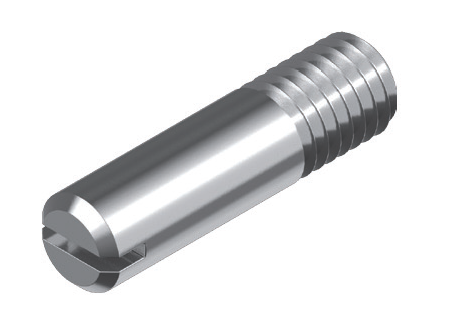
\includegraphics[height=3cm,width=1\textwidth,keepaspectratio]{pin_2.png}
                    % \caption{capture2}
                    \label{fig:pin_2.png}
                \end{subfigure}

                \begin{subfigure}{0.49\textwidth}
                    \centering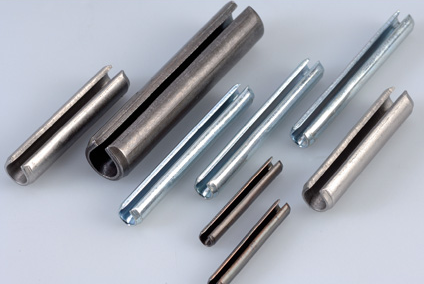
\includegraphics[height=3cm,width=1\textwidth,keepaspectratio]{pin_3.png}
                    % \caption{capture3}
                    \label{fig:pin_3.png}
                \end{subfigure}
                \begin{subfigure}{0.49\textwidth}
                    \centering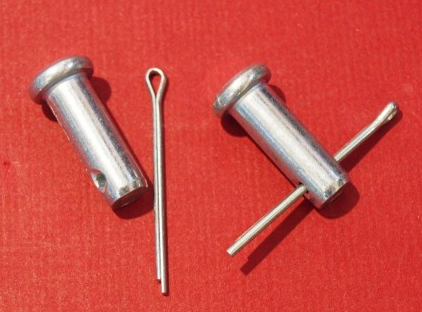
\includegraphics[height=3cm,width=1\textwidth,keepaspectratio]{pin_4.png}
                    % \caption{capture4}
                    \label{fig:pin_4.png}
                \end{subfigure}
            \end{figure}
        \end{column}
        \begin{column}{0.29\textwidth}
            \vspace{1cm}
            \begin{figure}[H]
                \centering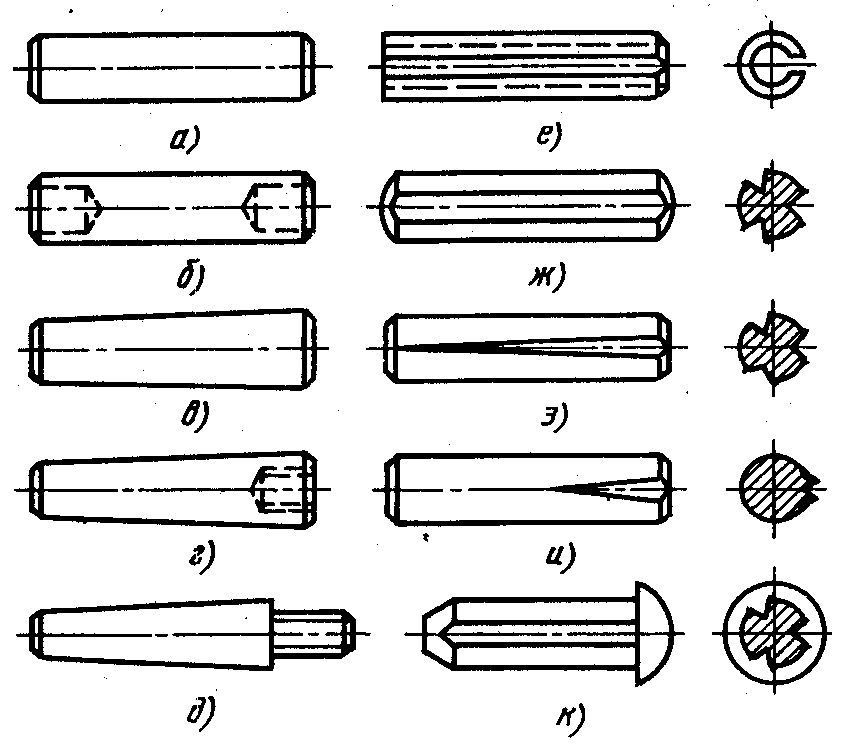
\includegraphics[height=5cm,width=1\textwidth,keepaspectratio]{types_of_pin.png}
                % \caption{caption_name}
                \label{fig:types_of_pin.png}
            \end{figure}
        \end{column}
    \end{columns}
\end{frame}

\begin{frame}[t]{Pin connections: applications}
    \framesubtitle{}
    \vspace{-0.6cm}
    \begin{figure}[H]
        \begin{subfigure}{0.49\textwidth}
            \centering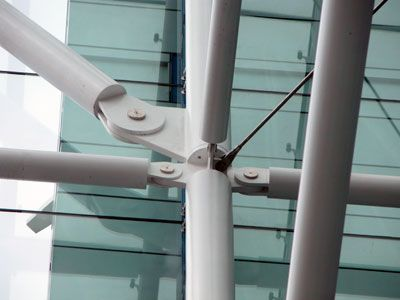
\includegraphics[height=2.5cm,width=1\textwidth,keepaspectratio]{pin_use_1.png}
            \caption*{Common usage}
            \label{fig:pin_use_1.png}
        \end{subfigure}
        \begin{subfigure}{0.49\textwidth}
            \centering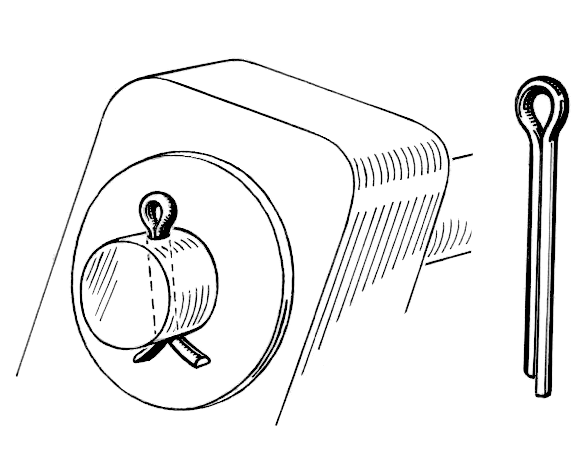
\includegraphics[height=2.5cm,width=1\textwidth,keepaspectratio]{pin_use_2.png}
            \caption*{Splint pin (Шплинтовое)}
            \label{fig:pin_use_2.png}
        \end{subfigure}

        \begin{subfigure}{0.49\textwidth}
            \centering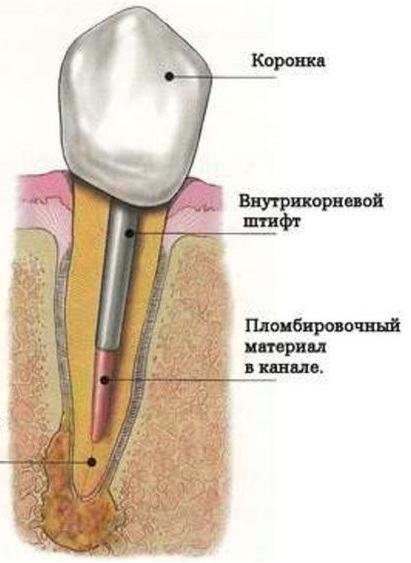
\includegraphics[height=2.5cm,width=1\textwidth,keepaspectratio]{pin_use_3.jpg}
            \caption*{Stomatology}
            \label{fig:pin_use_3.jpg}
        \end{subfigure}
        \begin{subfigure}{0.49\textwidth}
            \centering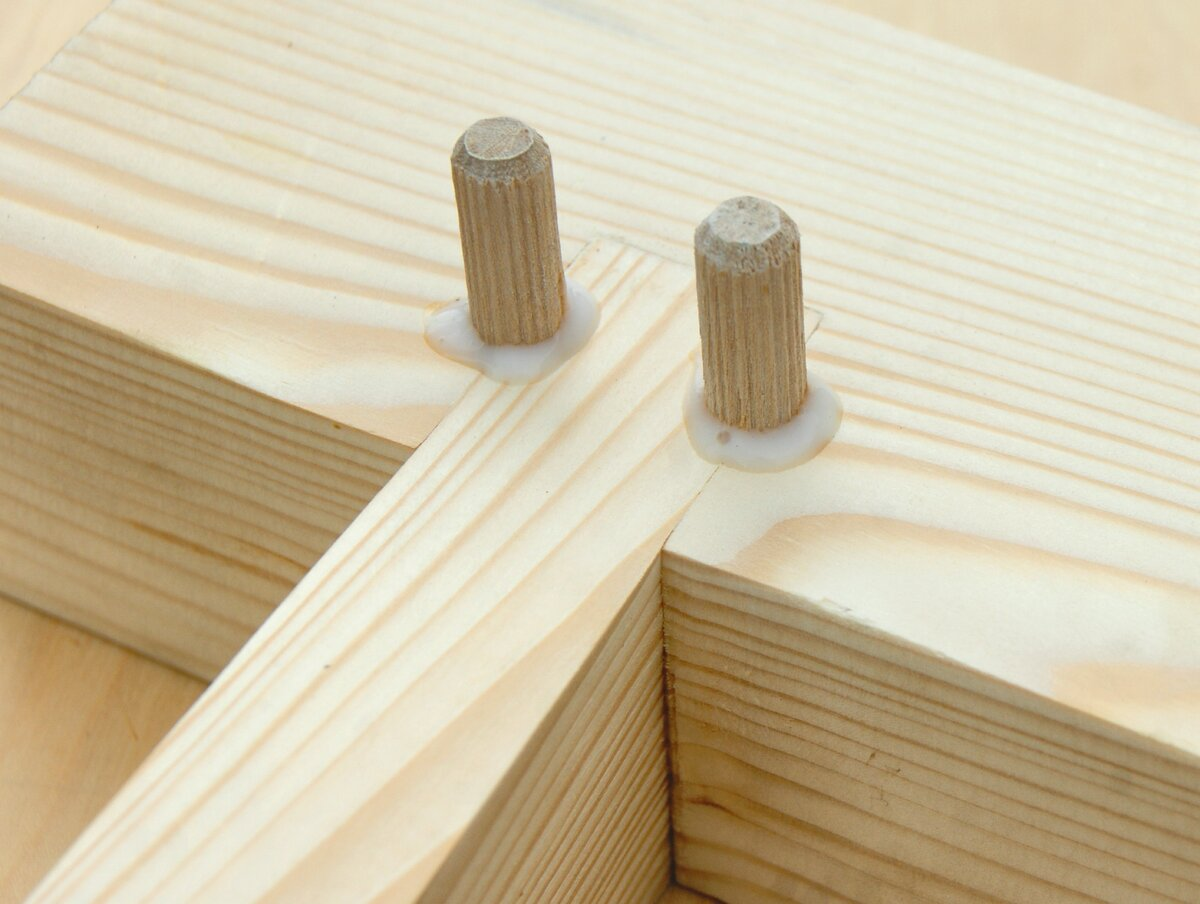
\includegraphics[height=2.5cm,width=1\textwidth,keepaspectratio]{dowel.jpeg}
            \caption*{Dowel (Шкант)}
            \label{fig:dowel.jpeg}
        \end{subfigure}
    \end{figure}
\end{frame}

\begin{frame}[t]{Pin types}
    \framesubtitle{Video}
    \vspace{-0.6cm}
    \begin{figure}[H]
        \href{https://youtu.be/W-0ZV9zXpc0}{
            \centering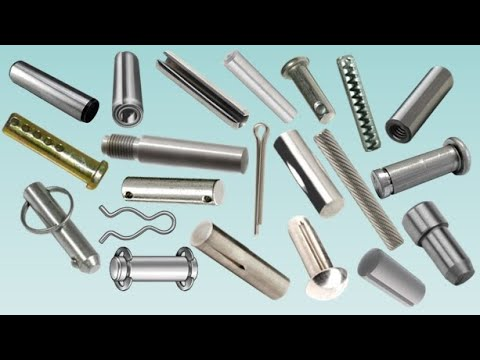
\includegraphics[height=6cm,width=1\textwidth,keepaspectratio]{pin_types_video.jpg}}
        \label{fig:pin_types_video.jpg}
    \end{figure}
\end{frame}

\begin{frame}[t]{Split Pin (Шплинтовое)}
    \framesubtitle{Video}
    \vspace{-0.6cm}
    \begin{figure}[H]
        \href{https://youtu.be/SpY0tJMY0hg}{
            \centering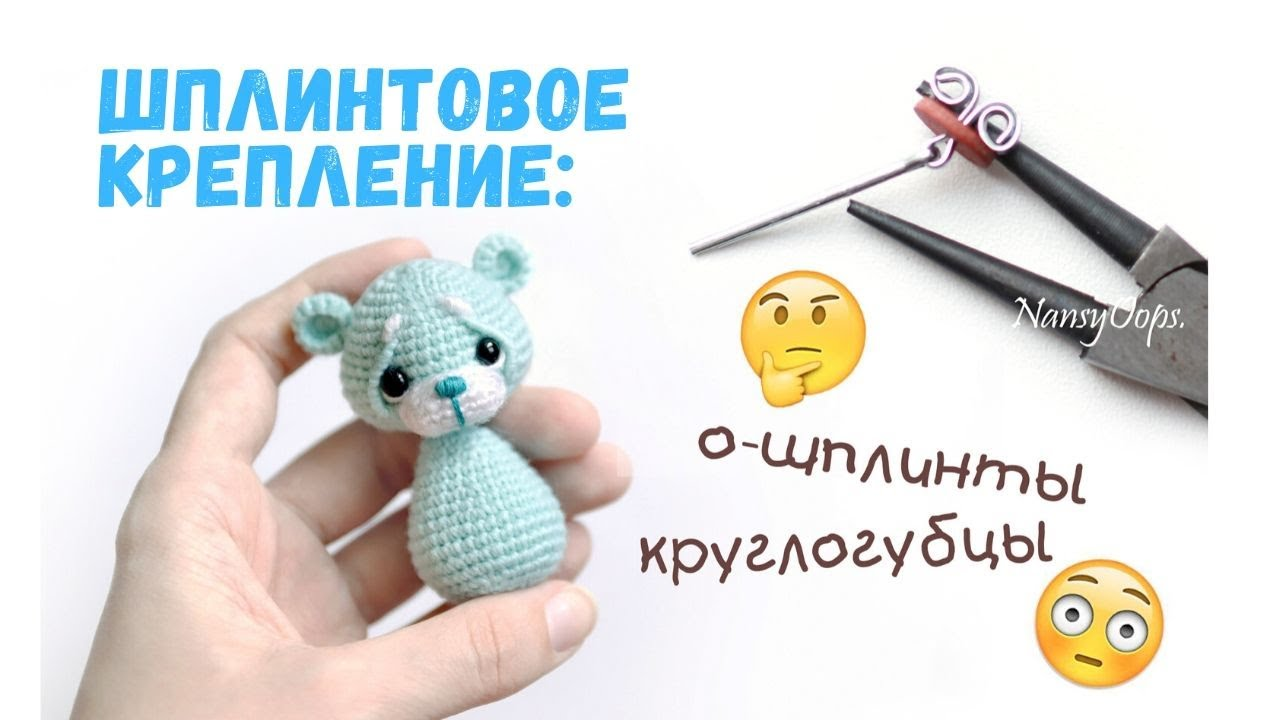
\includegraphics[height=6cm,width=1\textwidth,keepaspectratio]{splint_pin_video.jpg}}
        \label{fig:splint_pin_video.jpg}
    \end{figure}
\end{frame}

\begin{frame}[t]{Tongue \& Groove (Шпунт), Mortise \& Tenon (Шиповое)}
    \framesubtitle{}
    \begin{figure}[H]
        \begin{subfigure}{0.49\textwidth}
            \centering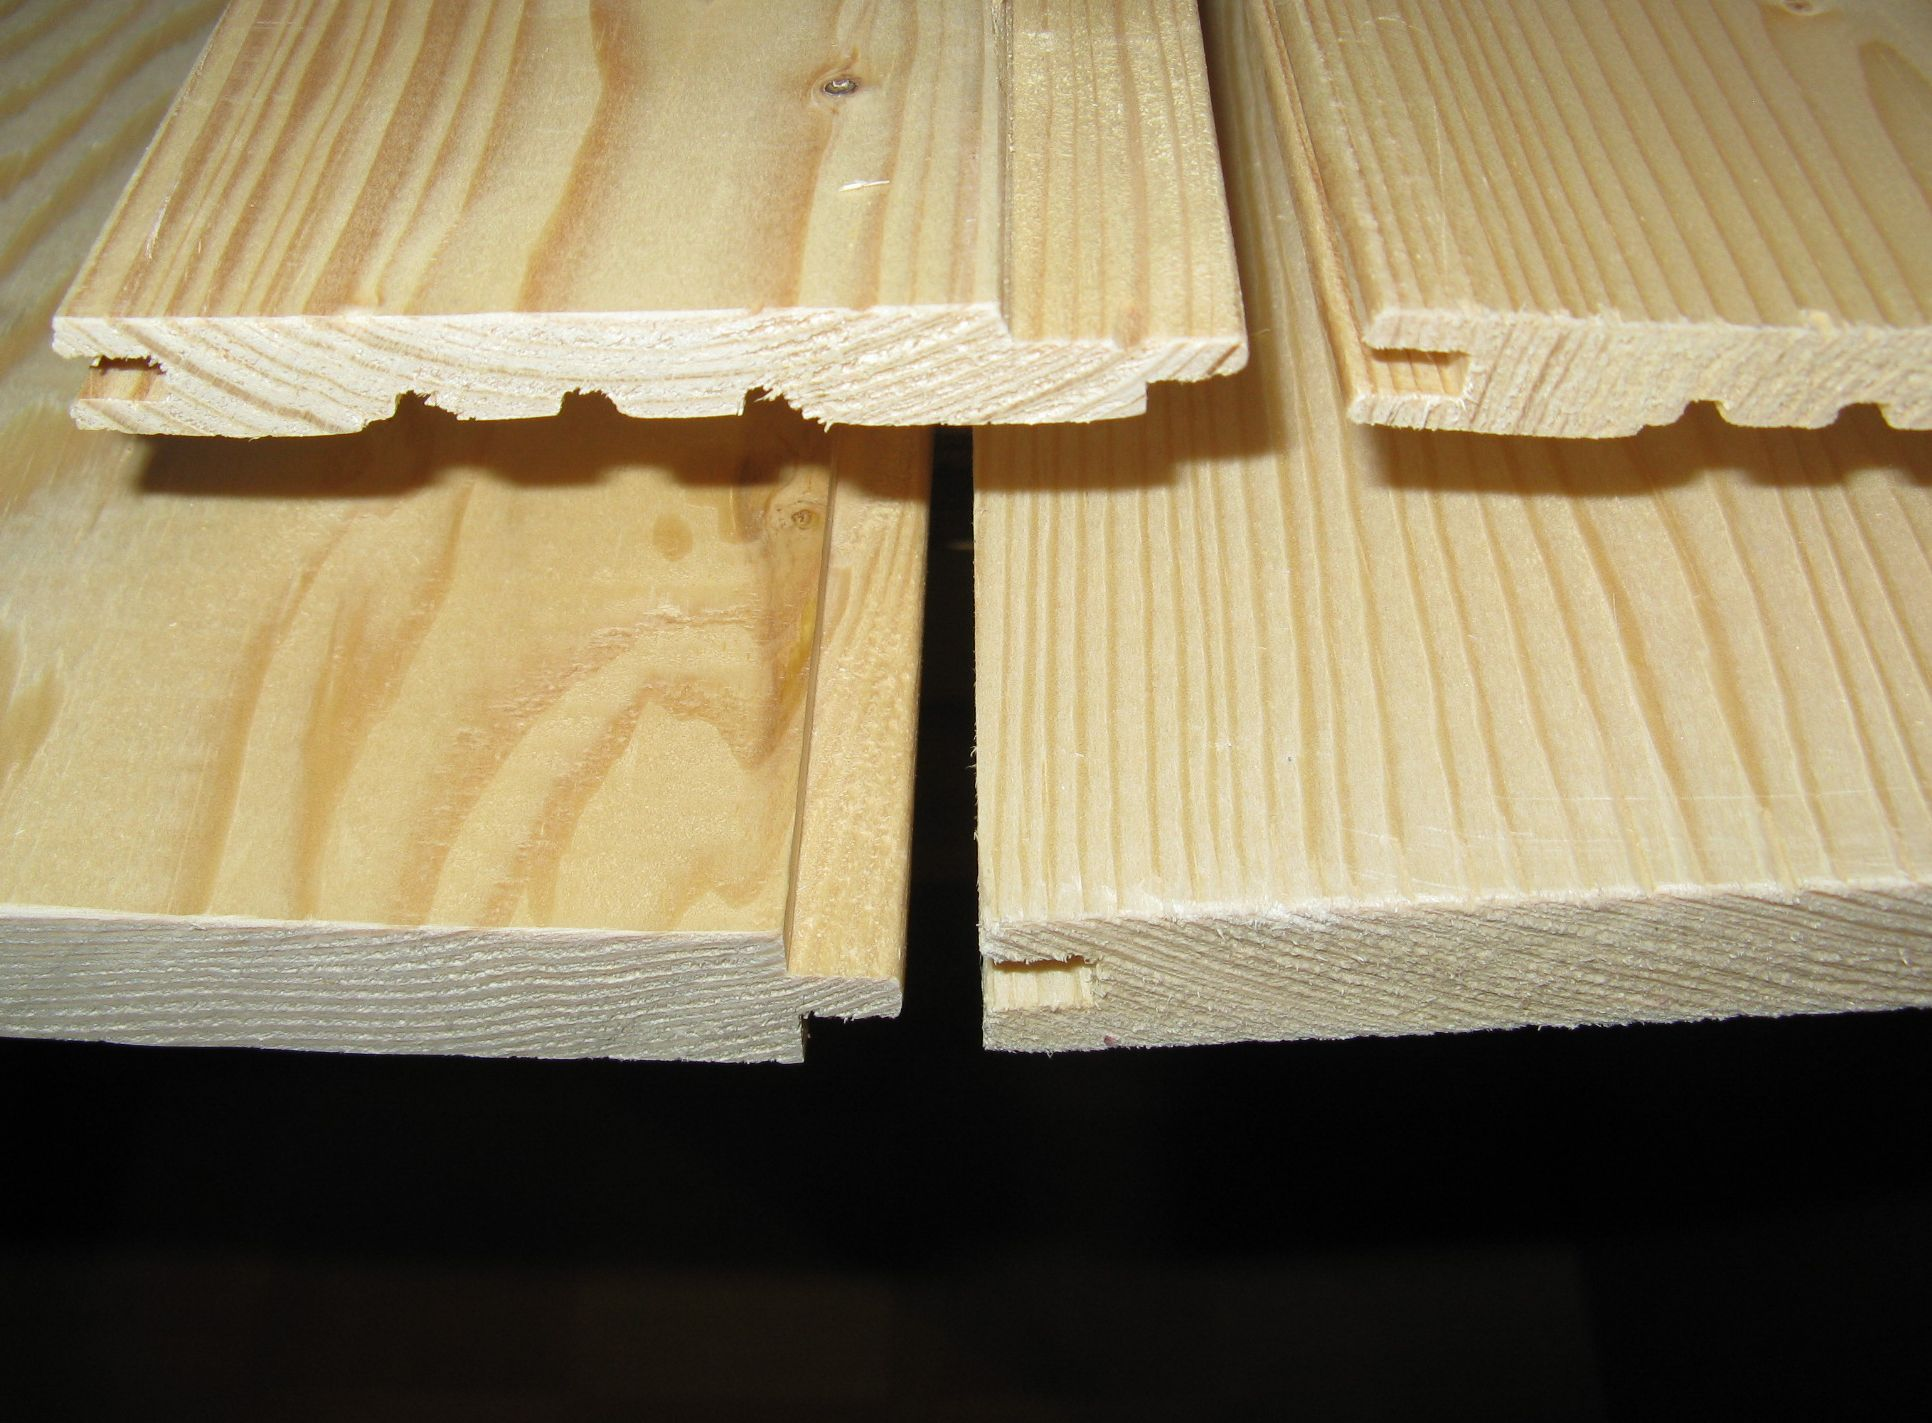
\includegraphics[height=5cm,width=1\textwidth,keepaspectratio]{spund.jpg}
            \caption*{Tongue and Groove (Шпунт)}
            \label{fig:spund.jpg}
        \end{subfigure}
        \begin{subfigure}{0.49\textwidth}
            \centering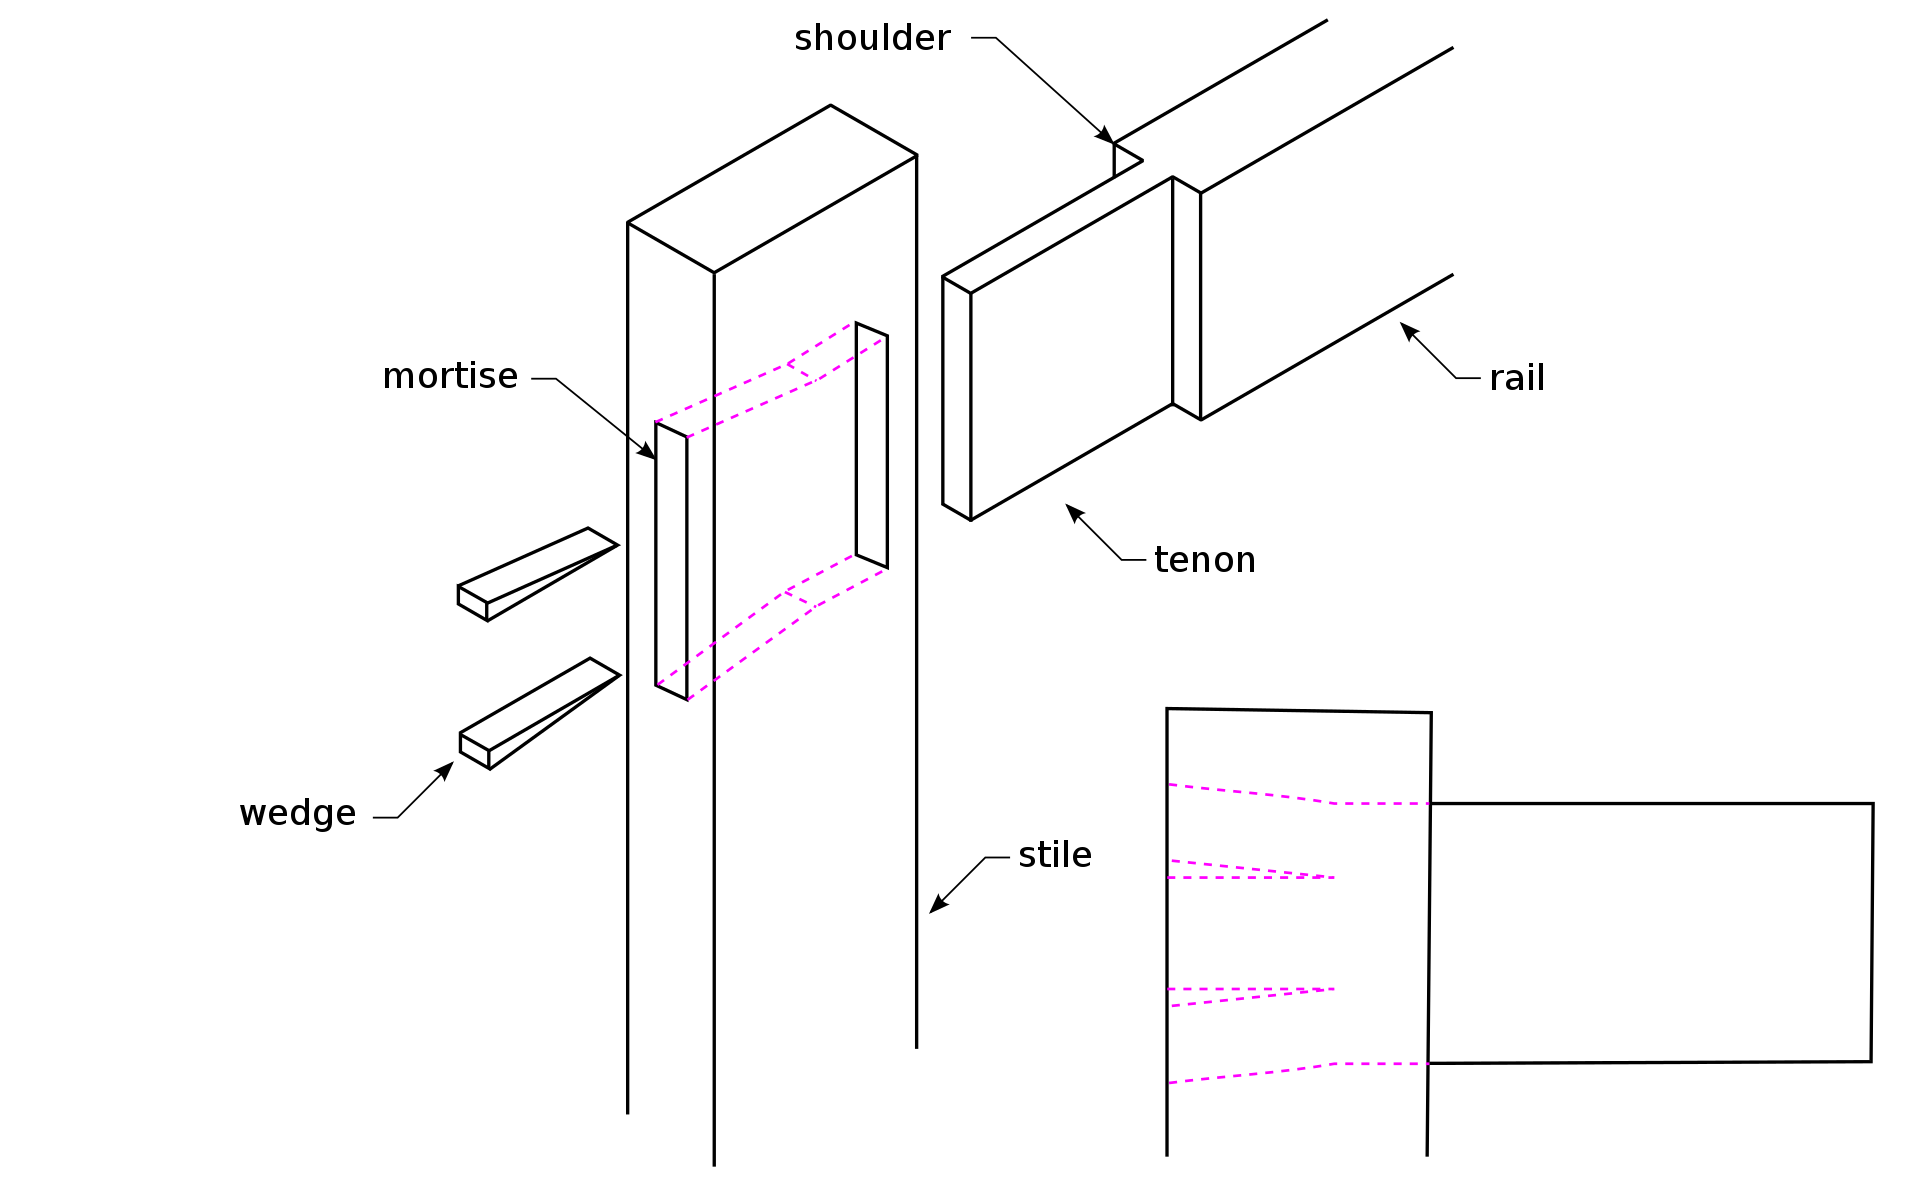
\includegraphics[height=6cm,width=1\textwidth,keepaspectratio]{Mortise.png}
            \caption*{Mortise and Tenon (Шиповое)}
            \label{fig:Mortise.png}
        \end{subfigure}
    \end{figure}
\end{frame}

\begin{frame}[t]{Threaded connection}
    \framesubtitle{}
    \begin{columns}[T,onlytextwidth]
        \begin{column}{0.49\textwidth}
            A bolted joint consists of a male threaded fastener (e. g., a bolt) that captures and joins other parts, secured with a matching female screw thread.
        \end{column}
        \begin{column}{0.49\textwidth}
            \vspace{-1cm}
            \begin{figure}[H]
                \begin{subfigure}{0.99\textwidth}
                    \centering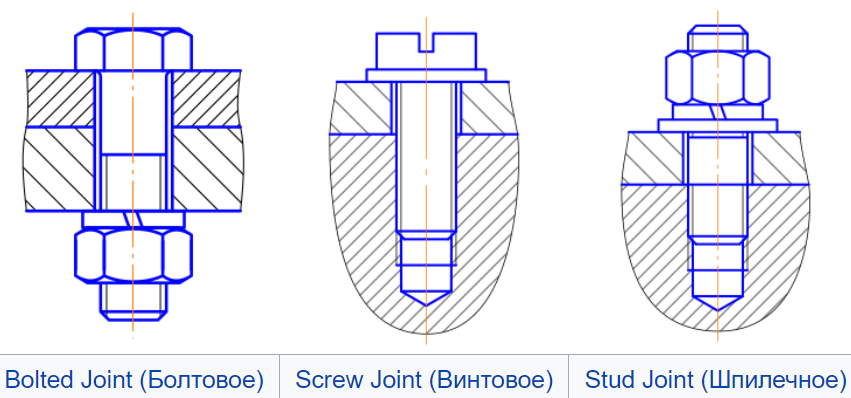
\includegraphics[height=3cm,width=1\textwidth,keepaspectratio]{threaded_types.png}
                    \label{fig:threaded_types.png}
                \end{subfigure}
                \begin{subfigure}{0.99\textwidth}
                    \centering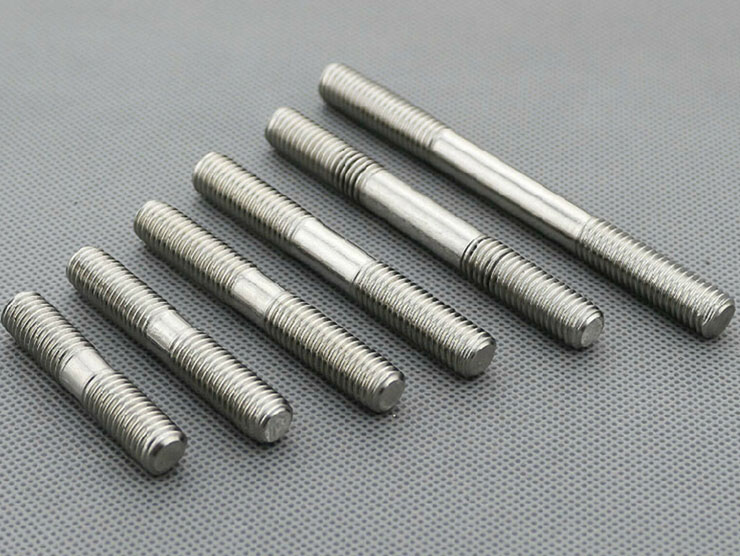
\includegraphics[height=3cm,width=1\textwidth,keepaspectratio]{studs.jpg}
                    \caption*{Studs}
                    \label{fig:studs.jpg}
                \end{subfigure}
            \end{figure}
        \end{column}
    \end{columns}
\end{frame}

\begin{frame}[t]{What should we know about threaded connection}
    \framesubtitle{}
    \begin{enumerate}
        \item Terminology of screw threads
        \item Their types, features
        \item How to prepare a place for them correctly
        \item How to mount them
    \end{enumerate}
\end{frame}

\begin{frame}[t]{Terminology of screw threads}
    \framesubtitle{}
    \begin{figure}[H]
        \begin{subfigure}{0.49\textwidth}
            \centering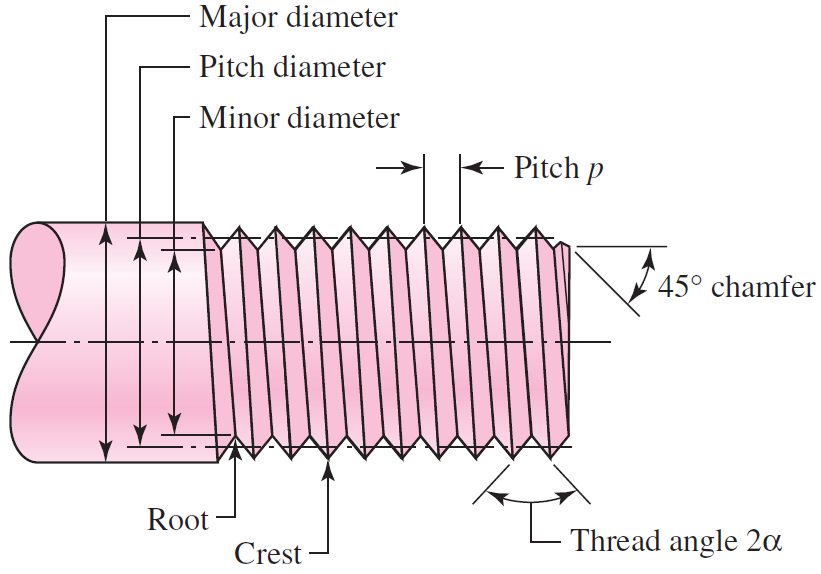
\includegraphics[height=5cm,width=1\textwidth,keepaspectratio]{screw_threads_terms.png}
            \label{fig:screw_threads_terms.png}
        \end{subfigure}
        \begin{subfigure}{0.49\textwidth}
            \centering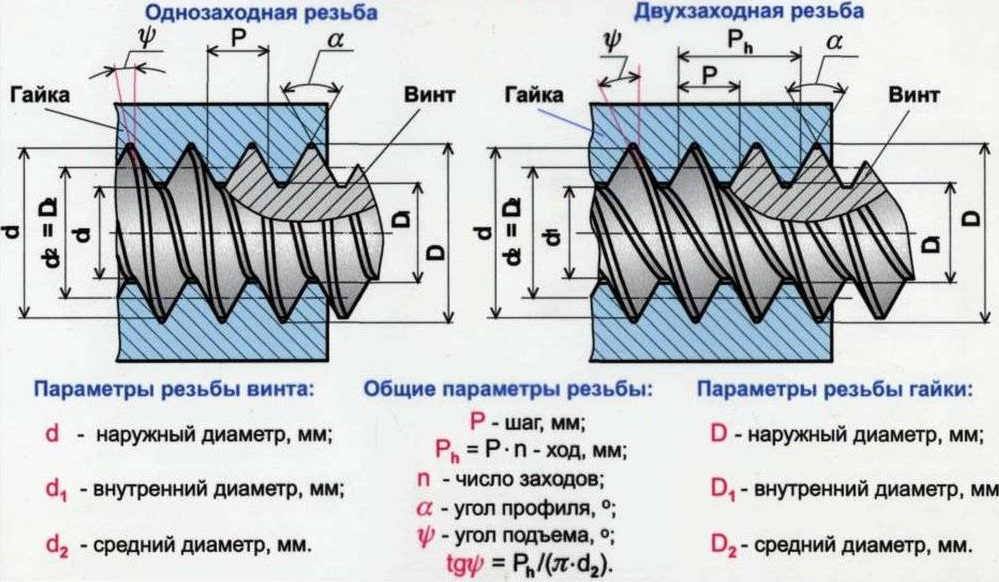
\includegraphics[height=5cm,width=1\textwidth,keepaspectratio]{geom_thread_param_rus.jpeg}
            \label{fig:geom_thread_param_rus.jpeg}
        \end{subfigure}
    \end{figure}
\end{frame}

\begin{frame}[t]{Thread Dimensions}
    \framesubtitle{}
    \vspace{-0.6cm}
    \begin{figure}[H]
        \centering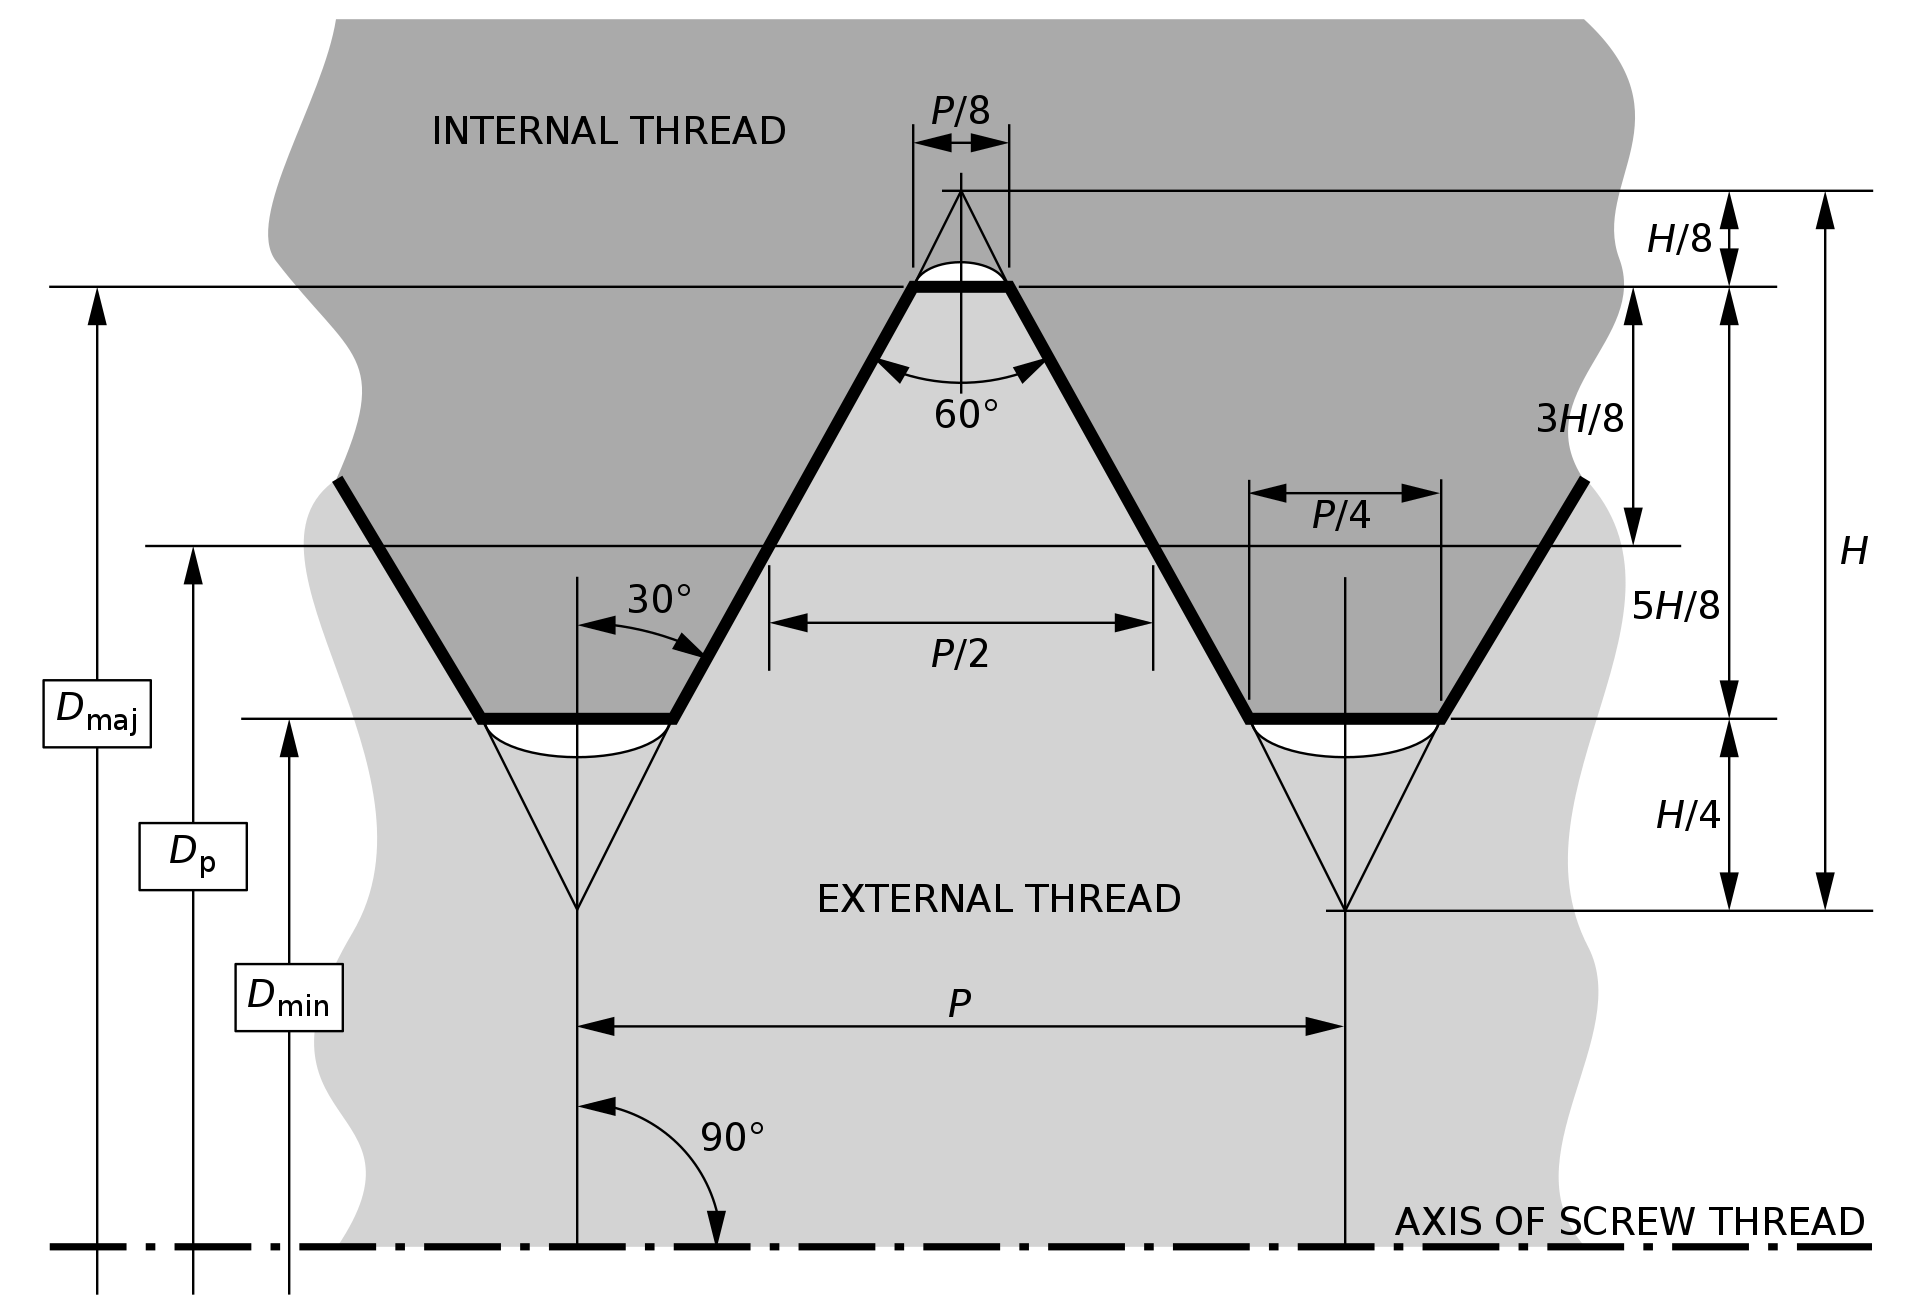
\includegraphics[height=6cm,width=1\textwidth,keepaspectratio]{thread_dimensions.png}
        \label{fig:thread_dimensions.png}
    \end{figure}
\end{frame}

\begin{frame}[t]{Multiple-Start thread}
    \framesubtitle{Video}
    \vspace{-0.6cm}
    \begin{figure}[H]
        \href{https://youtu.be/MwIBrNMjMrw}{
            \centering
\includegraphics[height=6cm,width=1\textwidth,keepaspectratio]{multitheding_video.jpg}}
        \label{fig:multitheding_video.jpg}
    \end{figure}
\end{frame}

\begin{frame}[t]{Magic Two-Sided screw}
    \framesubtitle{Video}
    \vspace{-0.6cm}
    \begin{figure}[H]
        \href{https://youtu.be/cDfMI5ahbJI?t=722}{
            \centering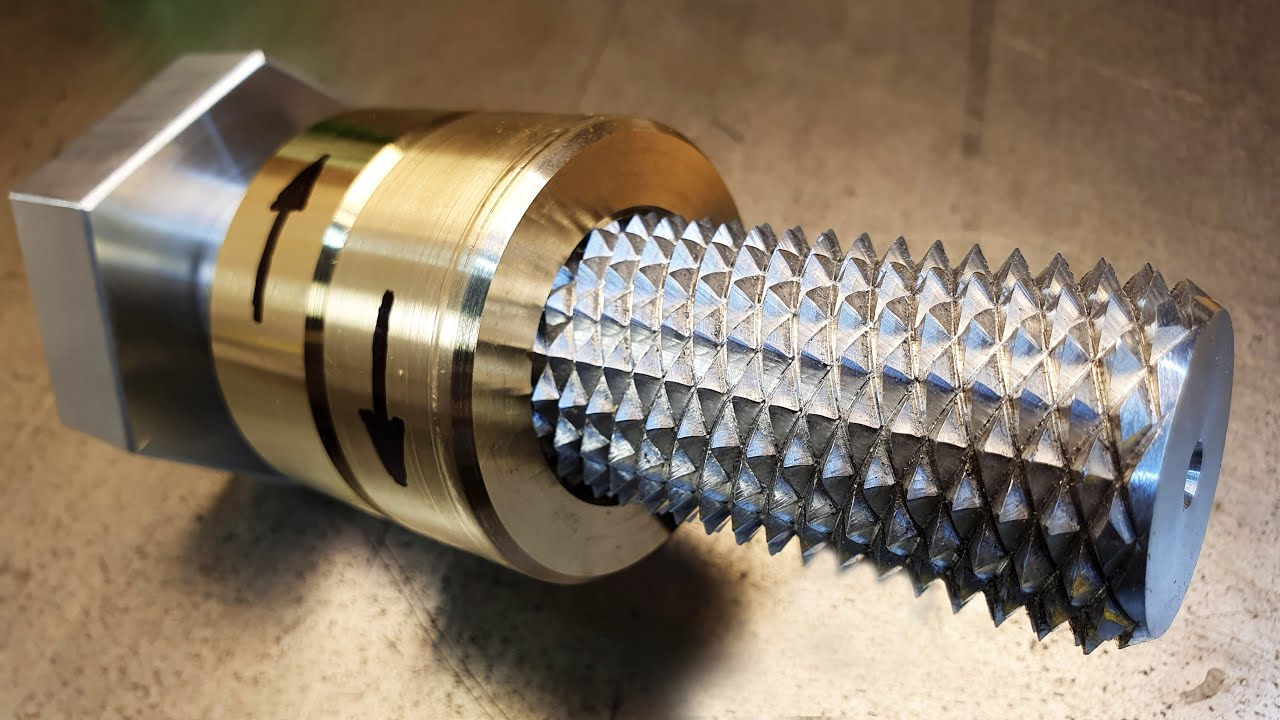
\includegraphics[height=6cm,width=1\textwidth,keepaspectratio]{two_sided_screw_video.jpg}}
        \label{fig:two_sided_screw_video.jpg}
    \end{figure}
\end{frame}

\begin{frame}[t]{Types of screws}
    \framesubtitle{Video}
    \vspace{-0.6cm}
    \begin{figure}[H]
        \href{https://youtu.be/Pe34Y-5LR9I}{
            \centering
\includegraphics[height=6cm,width=1\textwidth,keepaspectratio]{types_of_screws_video.jpg}}
        \label{fig:types_of_screws_video.jpg}
    \end{figure}
\end{frame}

\begin{frame}[t]{Difference between screws}
    \framesubtitle{}
    \vspace{-0.6cm}

    \begin{figure}[H]
        \begin{subfigure}{0.64\textwidth}
            \centering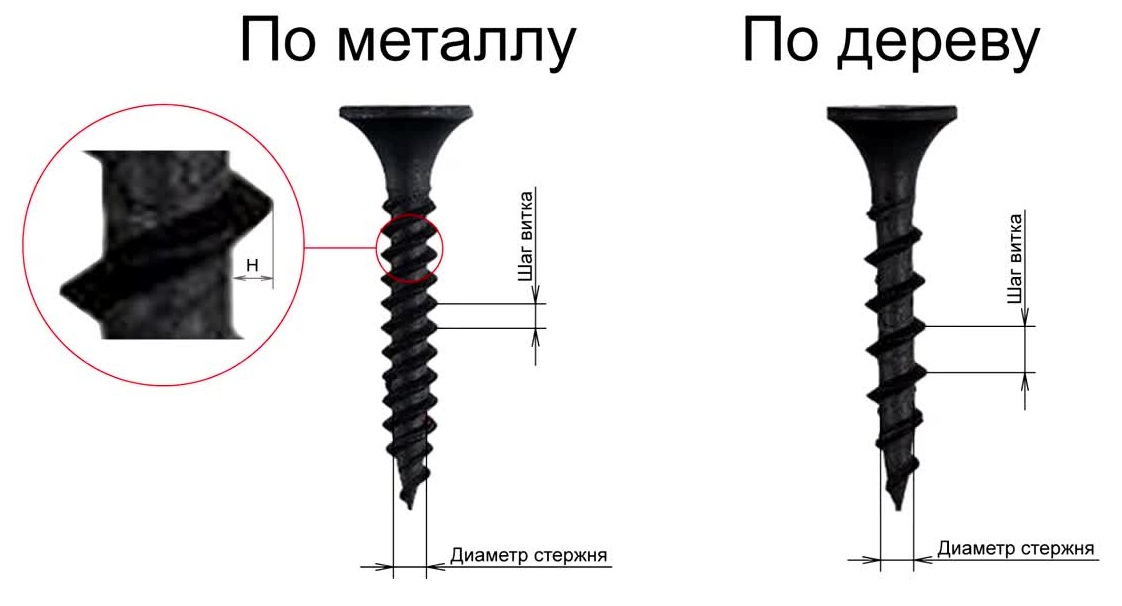
\includegraphics[height=6cm,width=1\textwidth,keepaspectratio]{diff_btw_screws.jpg}
            % \caption{capture1}
            \label{fig:diff_btw_screws.jpg}
        \end{subfigure}
        \begin{subfigure}{0.34\textwidth}
            \centering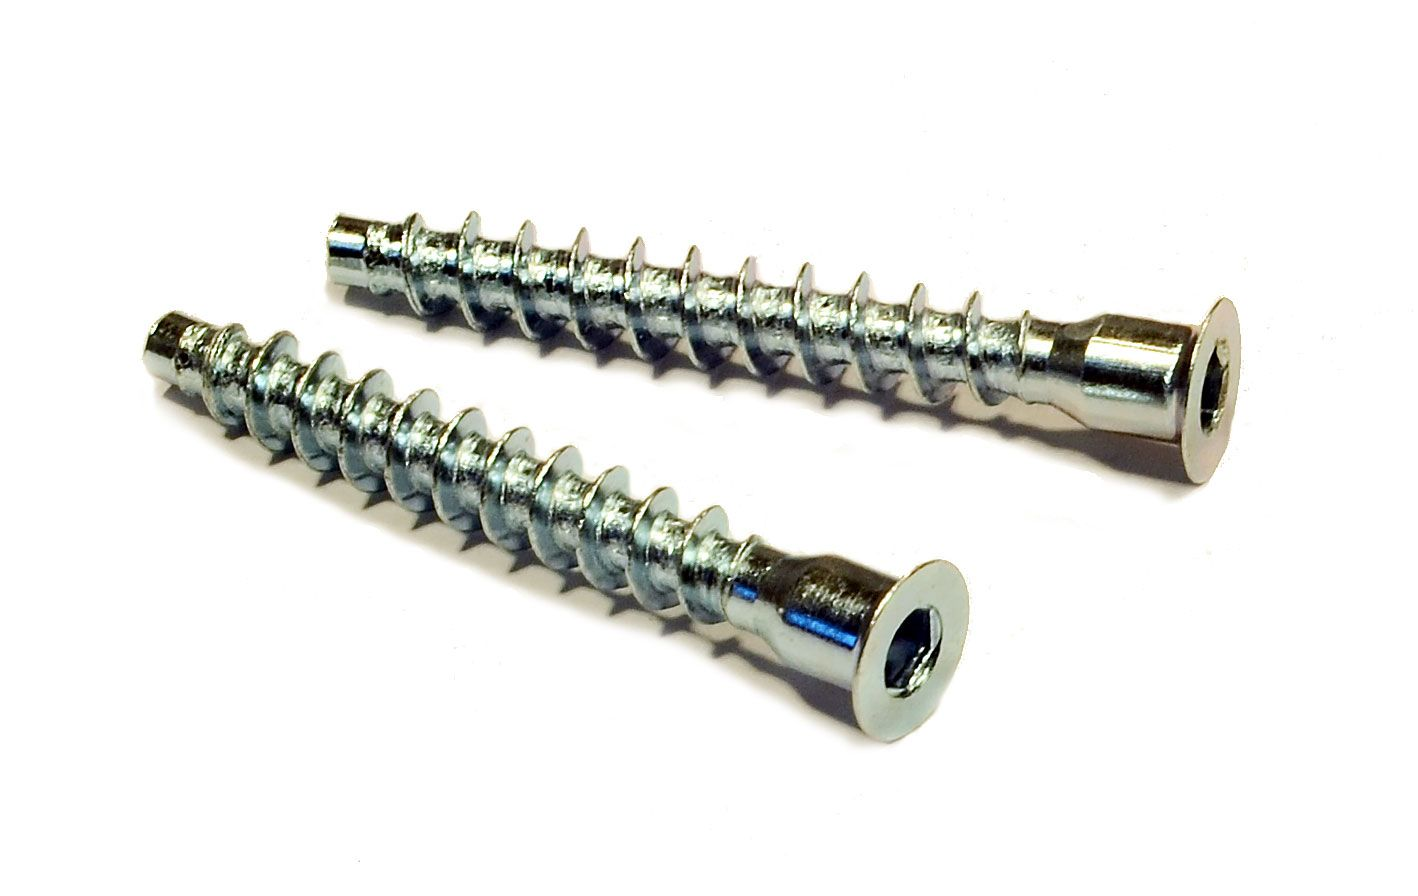
\includegraphics[height=6cm,width=1\textwidth,keepaspectratio]{komfirmat.jpg}
            \caption*{Confirmat (Конфирмат, Евровинт)}
            \label{fig:komfirmat.jpg}
        \end{subfigure}
    \end{figure}
\end{frame}


\begin{frame}[t]{Screw drive types (Шлицев)}
    \framesubtitle{}
    \vspace{-0.6cm}
    \begin{figure}[H]
        \centering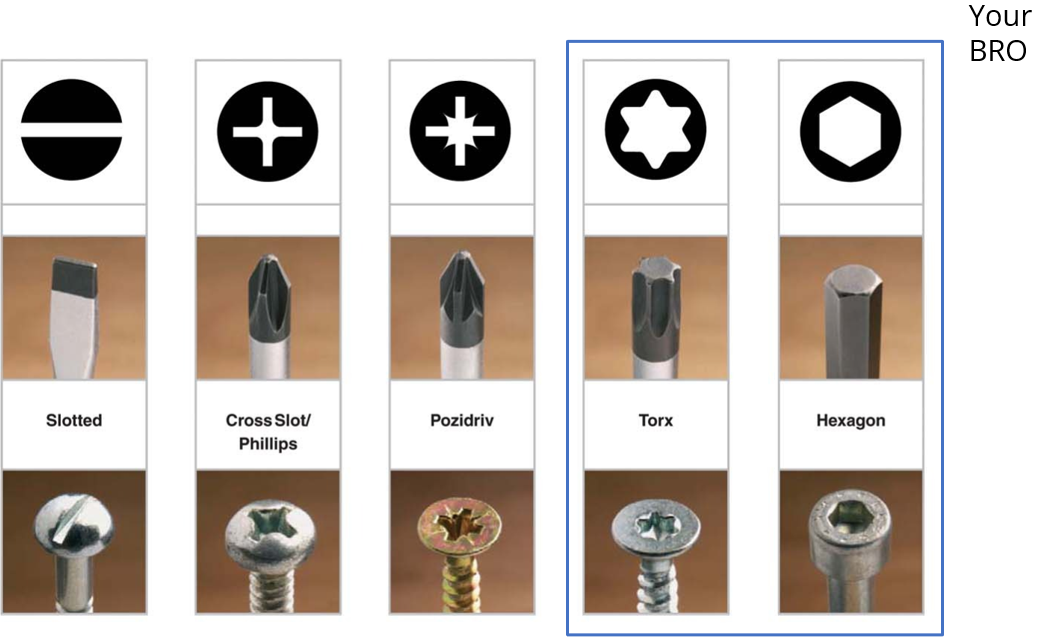
\includegraphics[height=6cm,width=1\textwidth,keepaspectratio]{screw_drive_types.png}
        \label{fig:screw_drive_types.png}
    \end{figure}
\end{frame}

\begin{frame}[t]{Site for ordering screws}
    \framesubtitle{Link to the site}
    \vspace{-0.6cm}
    \begin{figure}[H]
        \href{https://grover-sk.ru/catalog/metizy/}{
            \centering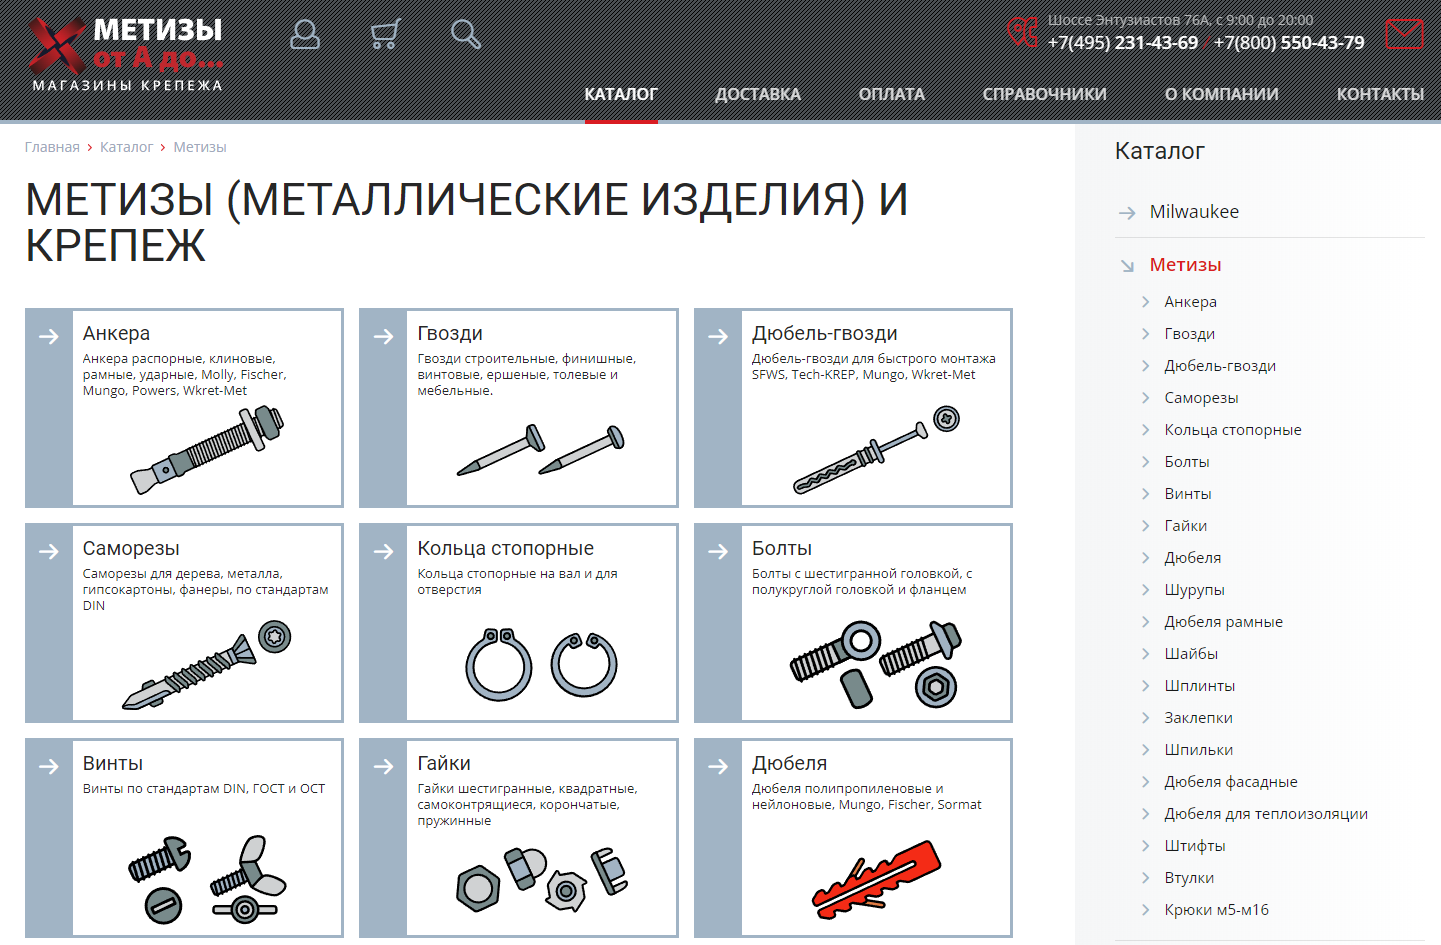
\includegraphics[height=6cm,width=1\textwidth,keepaspectratio]{metiz_site.png}}
        \label{fig:metiz_site.png}
    \end{figure}
\end{frame}

\begin{frame}[t]{Types of holes}
    \framesubtitle{}
    \vspace{-0.6cm}
    \begin{figure}[H]
        \begin{subfigure}{0.32\textwidth}
            \centering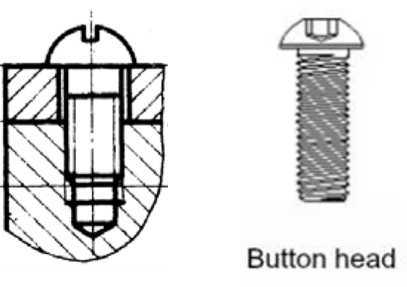
\includegraphics[height=6cm,width=1\textwidth,keepaspectratio]{common_hole.png}
            \caption*{Common hole (Отверстие)}
            \label{fig:common_hole.png}
        \end{subfigure}
        \begin{subfigure}{0.32\textwidth}
            \centering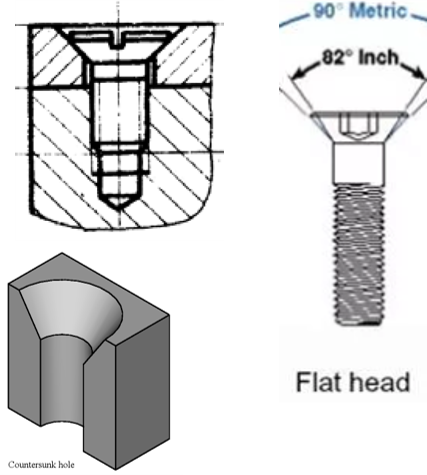
\includegraphics[height=6cm,width=1\textwidth,keepaspectratio]{countersunk_hole.png}
            \caption*{Countersunk hole (Зенкование)}
            \label{fig:countersunk_hole.png}
        \end{subfigure}
        \begin{subfigure}{0.32\textwidth}
            \centering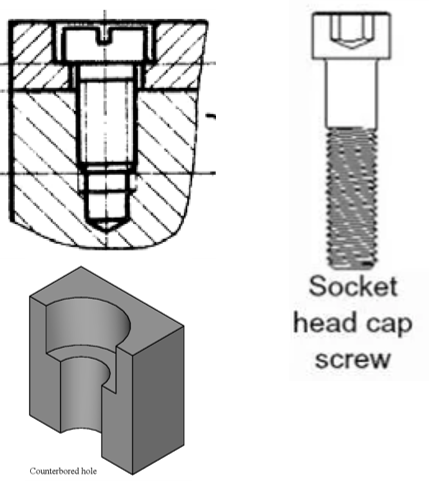
\includegraphics[height=6cm,width=1\textwidth,keepaspectratio]{counterbored_hole.png}
            \caption*{Counterbored hole (Цекование)}
            \label{fig:counterbored_hole.png}
        \end{subfigure}
    \end{figure}
\end{frame}

\begin{frame}[t]{Types of holes (drawings)}
    \framesubtitle{}
    \vspace{-0.6cm}
    \begin{figure}[H]
        \begin{subfigure}{0.32\textwidth}
            \centering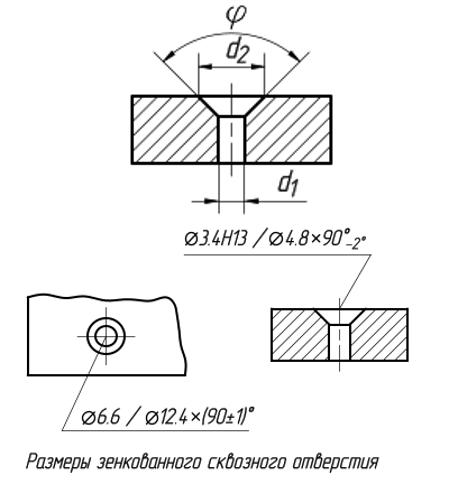
\includegraphics[height=6cm,width=1\textwidth,keepaspectratio]{countersunk_hole_drawing.png}
            \caption*{Countersunk hole (Зенкование)}
            \label{fig:countersunk_hole_drawing.png}
        \end{subfigure}
        \begin{subfigure}{0.32\textwidth}
            \centering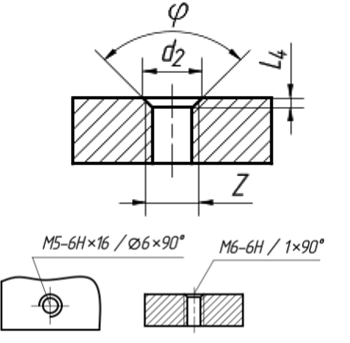
\includegraphics[height=6cm,width=1\textwidth,keepaspectratio]{thread_with_chamfer.png}
            \caption*{Thread with chamfer (c фаской)}
            \label{fig:thread_with_chamfer.png}
        \end{subfigure}
        \begin{subfigure}{0.32\textwidth}
            \centering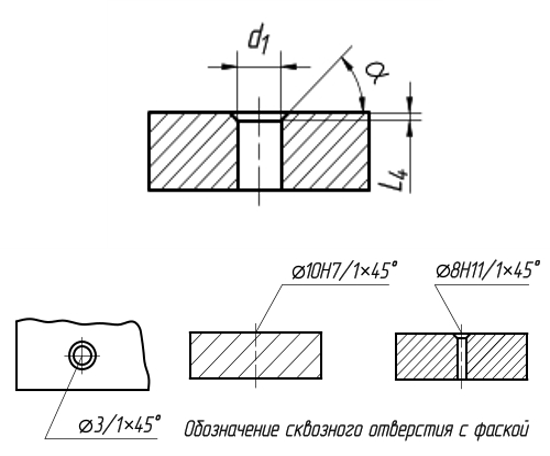
\includegraphics[height=6cm,width=1\textwidth,keepaspectratio]{hole_with_champfer.png}
            \caption*{Hole with chamfer}
            \label{fig:hole_with_champfer.png}
        \end{subfigure}
    \end{figure}
\end{frame}

\begin{frame}[t]{Type of drills}
    \framesubtitle{Video}
    \vspace{-0.6cm}
    \begin{figure}[H]
        \href{https://youtu.be/1TvtzPEFVIg}{
            \centering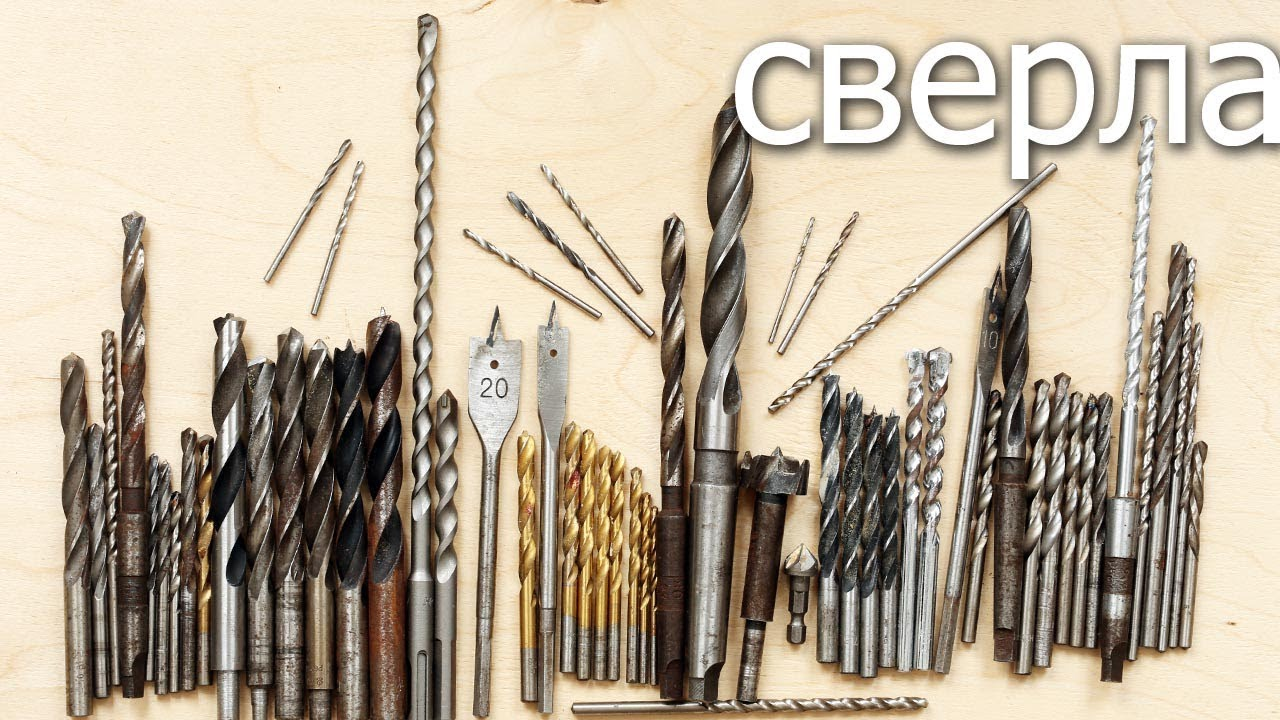
\includegraphics[height=6cm,width=1\textwidth,keepaspectratio]{type_of_drills_video.jpg}}
        \label{fig:type_of_drills_video.jpg}
    \end{figure}
\end{frame}

\begin{frame}[t]{Type of drills}
    \framesubtitle{}
    \vspace{-0.6cm}
    \begin{figure}[H]
        \centering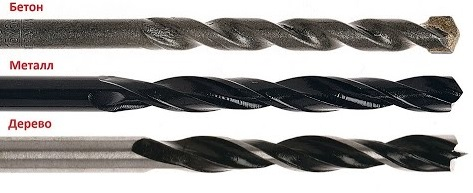
\includegraphics[height=6cm,width=1\textwidth,keepaspectratio]{types_of_drills.jpg}
        \label{fig:types_of_drills.jpg}
    \end{figure}
\end{frame}

\begin{frame}[t]{Threaded hole with a tap drill (мечИк)}
    \framesubtitle{Video}
    \vspace{-0.6cm}
    \begin{figure}[H]
        \href{https://youtu.be/PTlRTipSVNk?t=31}{
            \centering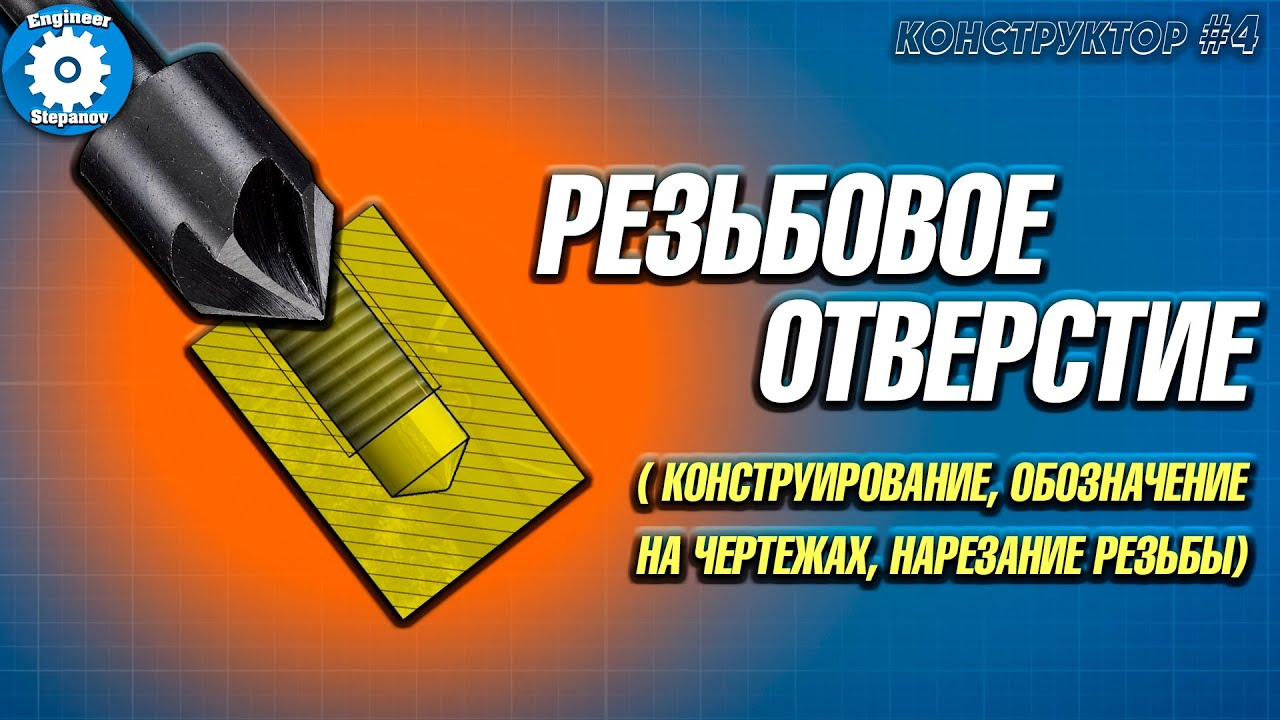
\includegraphics[height=6cm,width=1\textwidth,keepaspectratio]{threaded_hole_video.jpg}}
        \label{fig:threaded_hole_video.jpg}
    \end{figure}
\end{frame}

\begin{frame}[t]{How to make holes correctly}
    \framesubtitle{}
    \vspace{-0.6cm}
    \begin{figure}[H]
        \begin{subfigure}{0.59\textwidth}
            \centering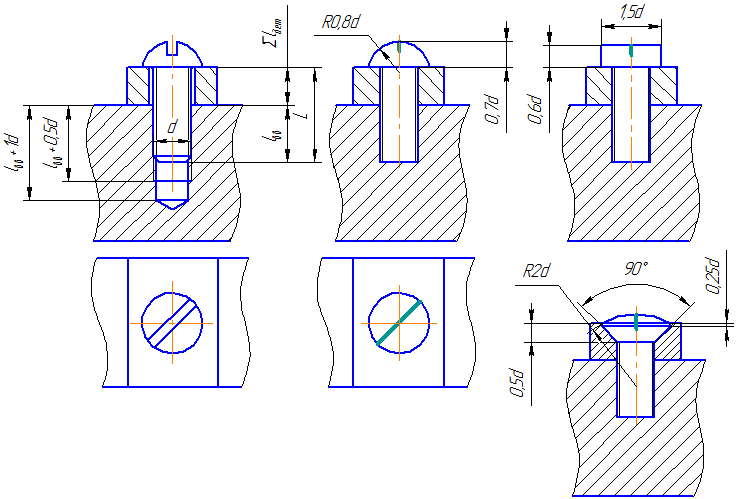
\includegraphics[height=6cm,width=1\textwidth,keepaspectratio]{vint_soed_2.png}
            \label{fig:vint_soed_2.png}
        \end{subfigure}
        \begin{subfigure}{0.39\textwidth}
            \centering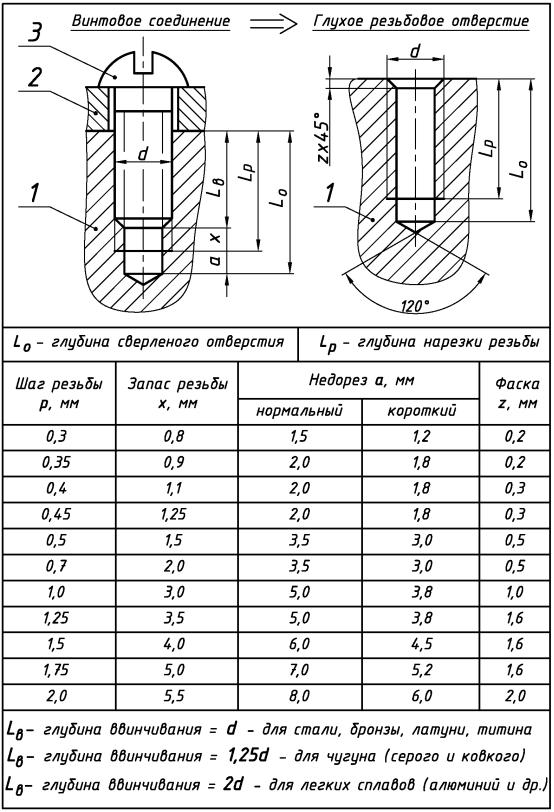
\includegraphics[height=6cm,width=1\textwidth,keepaspectratio]{gluh_thread.jpg}
            \label{fig:gluh_thread.jpg}
        \end{subfigure}
    \end{figure}
\end{frame}

\begin{frame}[t]{Clearances for hole}
\framesubtitle{Reference material}
        \vspace{-0.4cm}
        \begin{figure}[H]
            \begin{subfigure}[t]{0.48\textwidth}
                \centering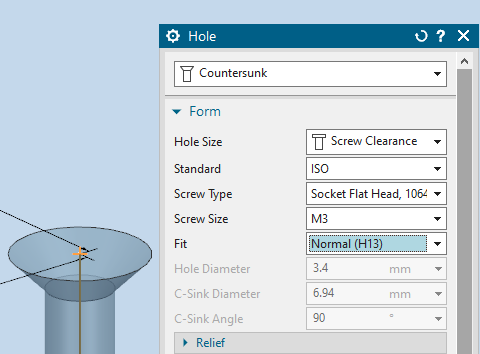
\includegraphics[height=4cm,width=1\textwidth,keepaspectratio]{nx_countersunk.png}
                % \caption{capture1}
                \label{fig:nx_countersunk.png}
            \end{subfigure}
            \begin{subfigure}[t]{0.48\textwidth}
                \centering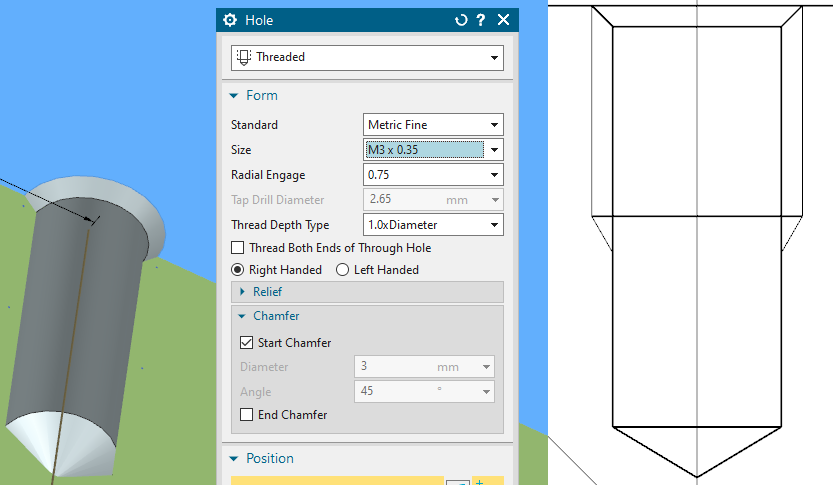
\includegraphics[height=4cm,width=1\textwidth,keepaspectratio]{nx_thread.png}
                % \caption{capture2}
                \label{fig:nx_thread.png}
            \end{subfigure}
        \end{figure}
        \vspace{-0.7cm}

        \begin{itemize}
            \item \href{https://engineersbible.com/clearance-hole-metric/}{Clearance Hole Size for Bolts and Screws (Metric)}
            \item \href{https://www.machiningdoctor.com/charts/metric-thread-charts/}{Tap drill size chart}
        \end{itemize}
\end{frame}

\begin{frame}[t]{Types of nuts (Гайки)}
    \framesubtitle{}
    \vspace{-0.6cm}
    \begin{figure}[H]
        \centering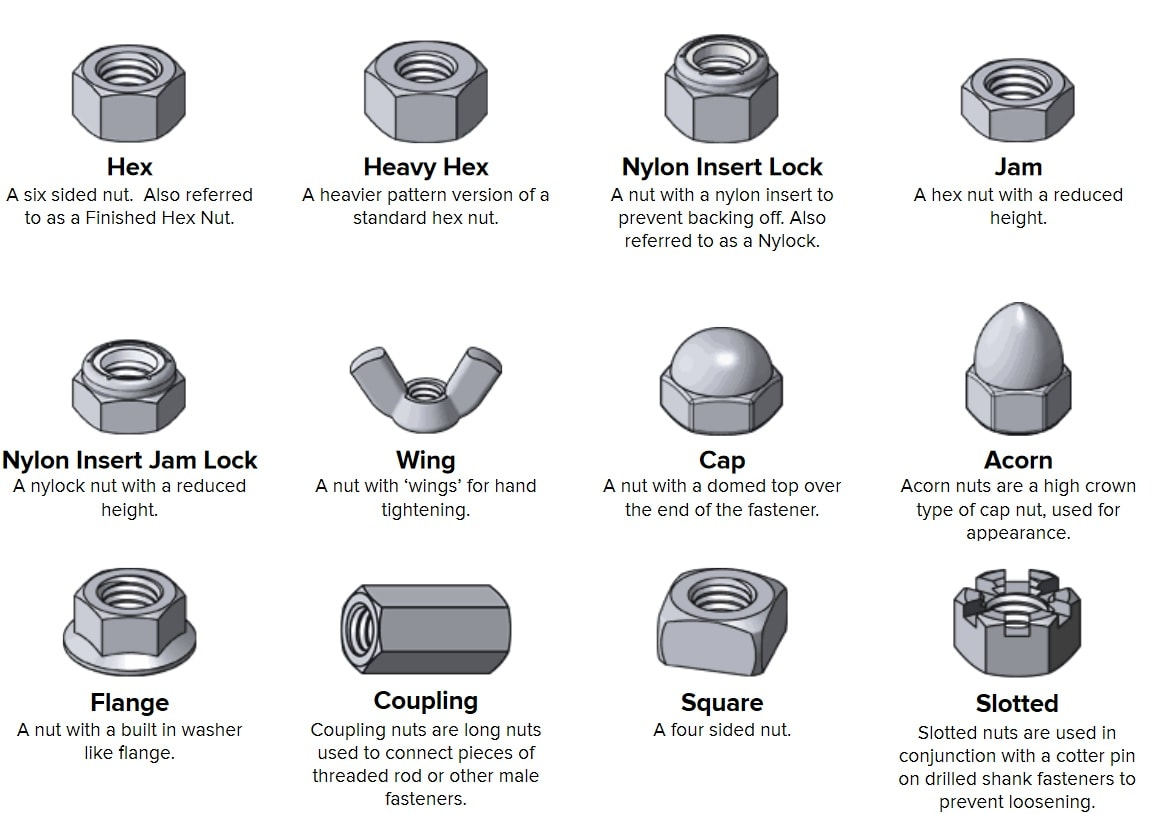
\includegraphics[height=6cm,width=1\textwidth,keepaspectratio]{nuts.jpg}
        \label{fig:nuts.jpg}
    \end{figure}
\end{frame}

\begin{frame}[t]{Types of washers (Шайбы)}
    \framesubtitle{}
    \vspace{-0.6cm}
    \begin{figure}[H]
        \centering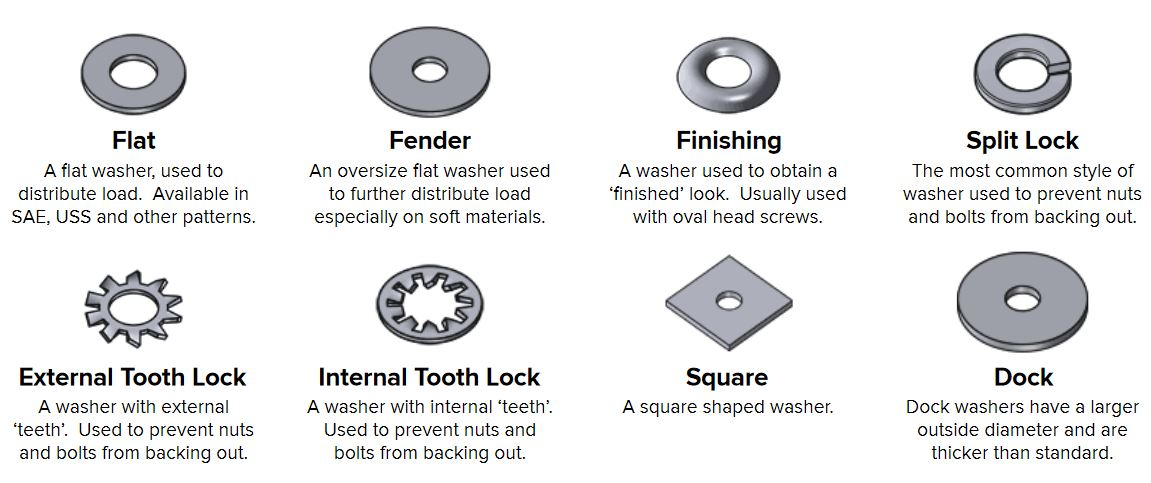
\includegraphics[height=6cm,width=1\textwidth,keepaspectratio]{washers.jpg}
        \label{fig:washers.jpg}
    \end{figure}
\end{frame}

\begin{frame}[t]{Threaded}
    \framesubtitle{Reference material}
    \begin{itemize}
        \item \href{https://youtu.be/LYUKs4LePc4}{Threaded connection (video, rus)}
        \item \href{https://steepmen.ru/mnogozakhodnaya-rezba/}{Multy start thread (rus)}
        \item \href{http://ng.sibstrin.ru/wolchin/umm/carving/carving/003.htm\#001}{Doc with all references to GOST (rus)}
        \item \href{https://cadinstructor.org/eg/lectures/5-2-krepegnie-izdeliya/\#5.515}{Nice material about holes (rus)}
        \item \href{https://youtu.be/lbIHMyxHkds}{Four common washer types and uses (video)}
    \end{itemize}
\end{frame}

\begin{frame}[t]{Glued (Adhesive) (Клеевое)}
    \framesubtitle{}
    \begin{columns}[T,onlytextwidth]
        \begin{column}{0.49\textwidth}
            Adhesive, also known as glue is any non-metallic substance applied to one or both surfaces of two separate items that binds them together and resists their separation.

            The use of adhesives offers certain advantages over other binding techniques such as sewing, mechanical fastenings, or welding.
        \end{column}
        \begin{column}{0.49\textwidth}
            \begin{figure}[H]
                \centering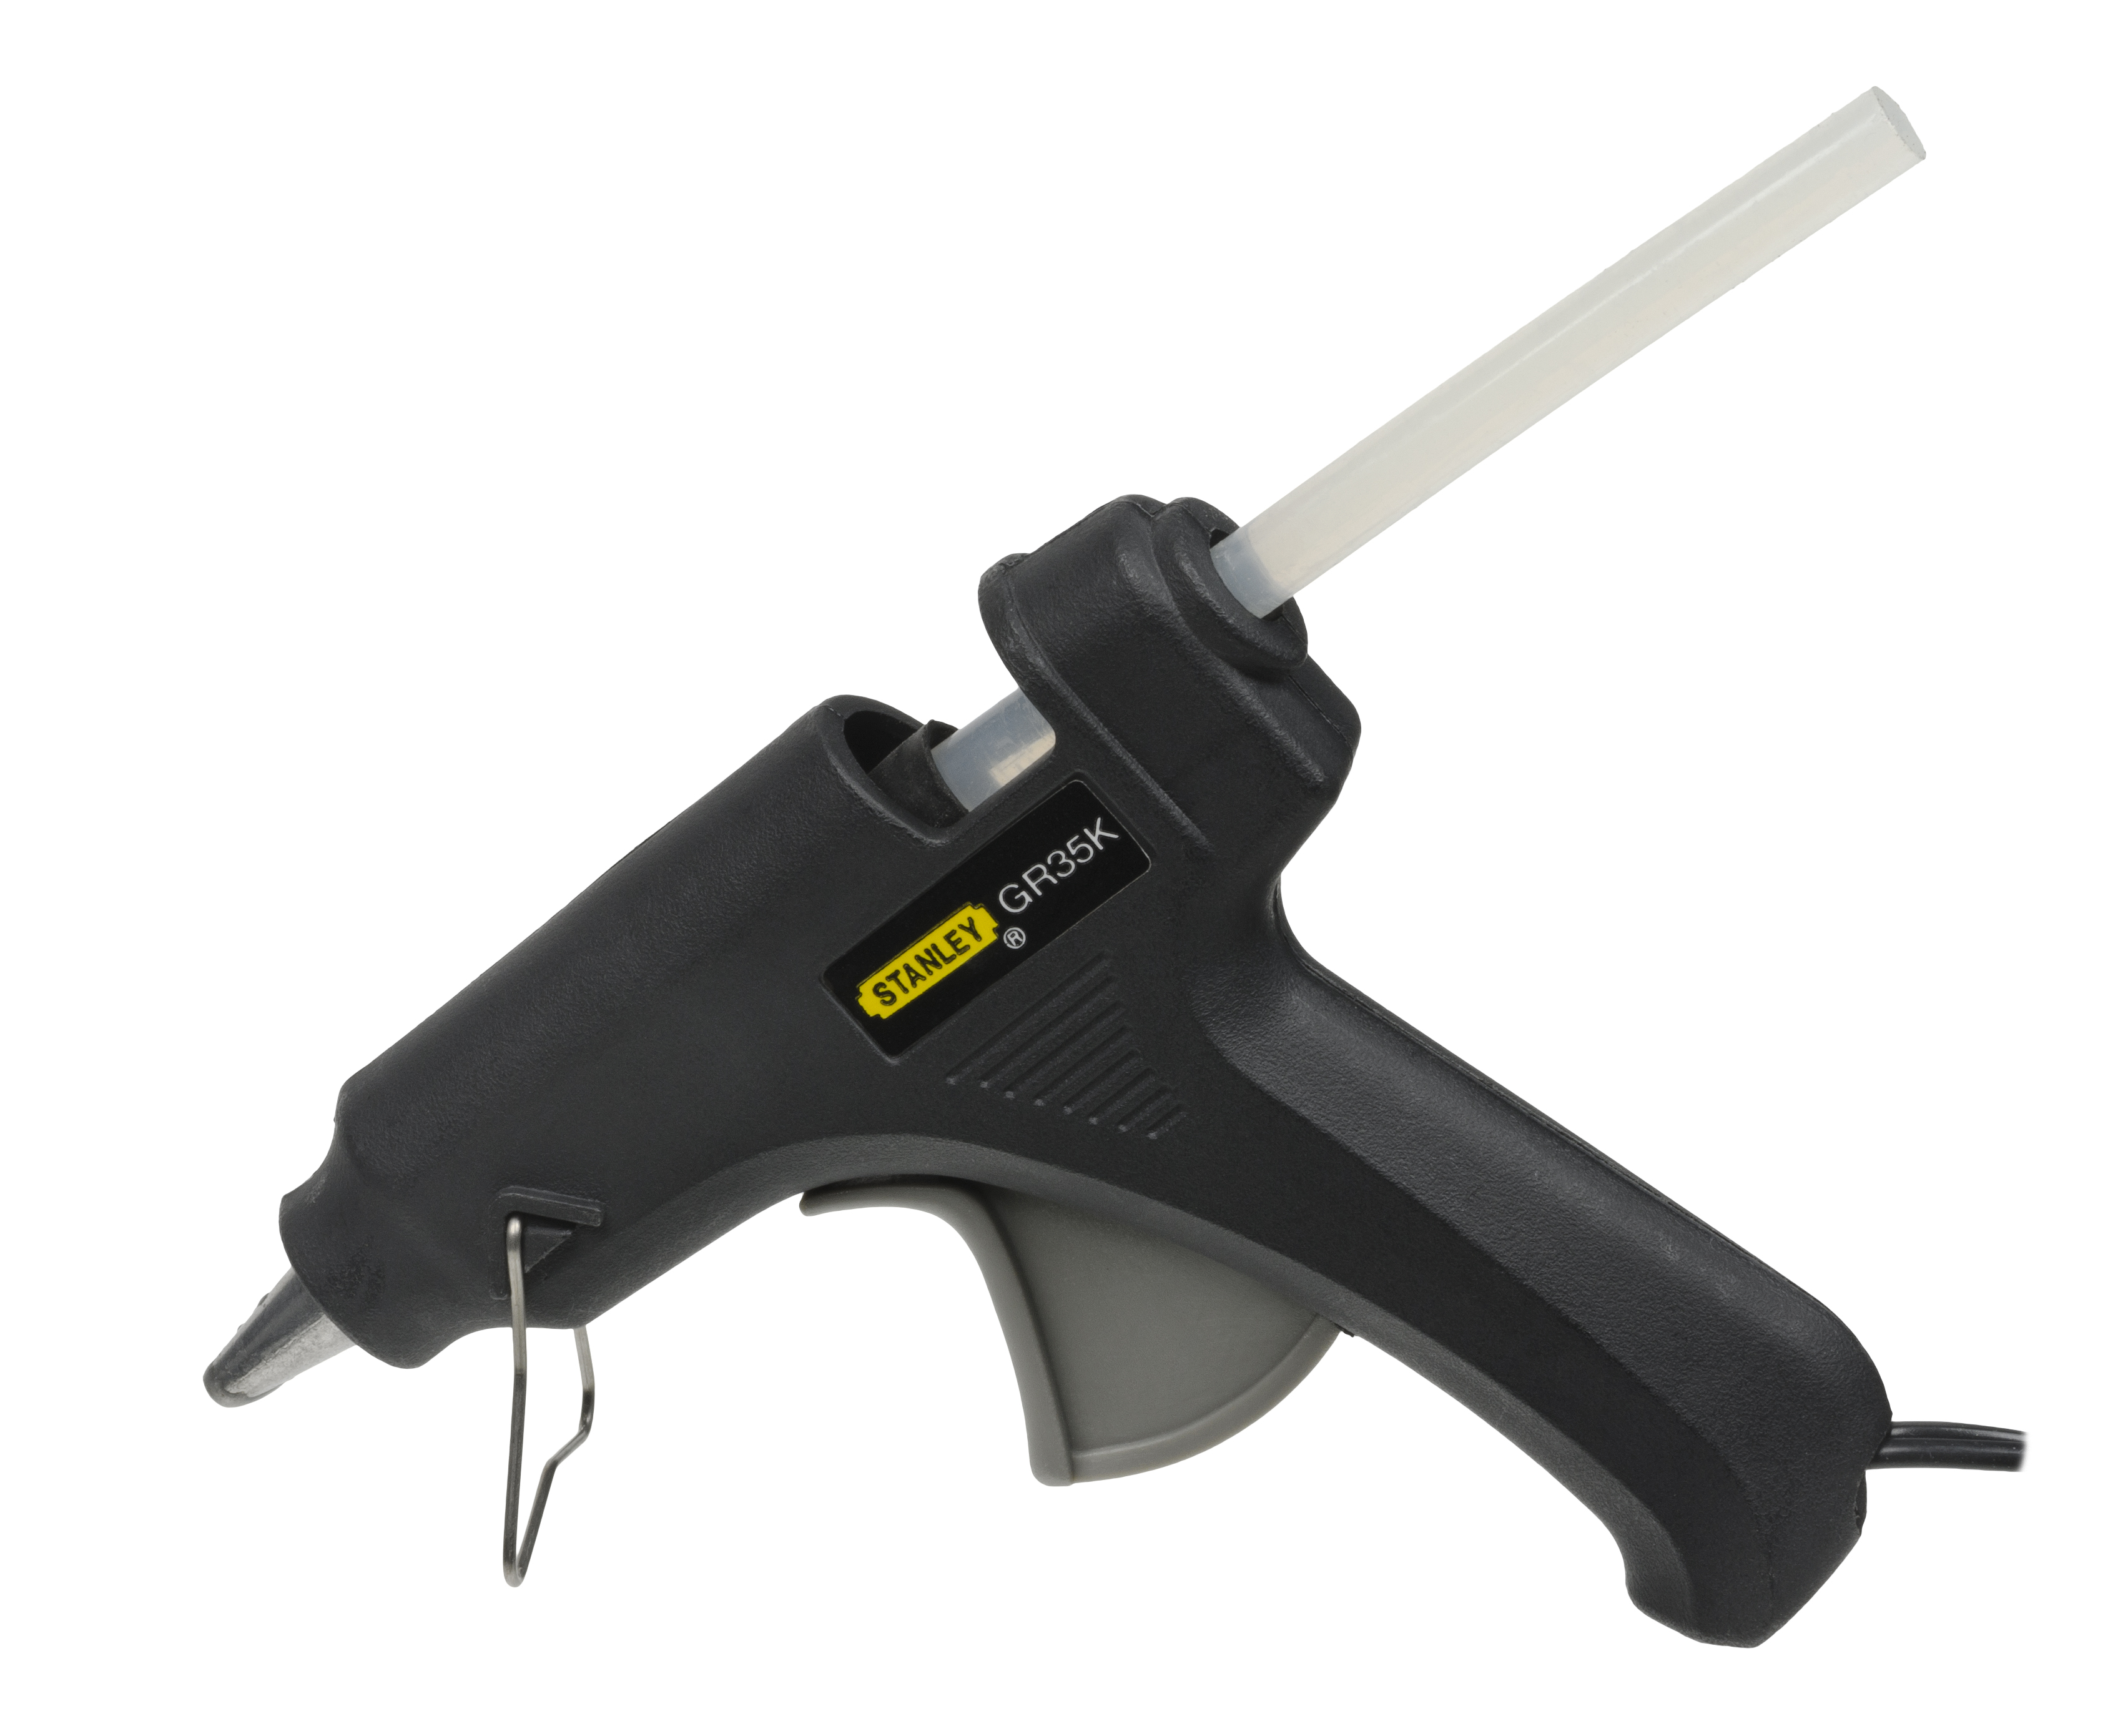
\includegraphics[height=5cm,width=1\textwidth,keepaspectratio]{glue_gun.jpg}
                % \caption{caption_name}
                \label{fig:glue_gun.jpg}
            \end{figure}
        \end{column}
    \end{columns}
\end{frame}

\begin{frame}[t]{Glues for wood}
    \framesubtitle{Video}
    \vspace{-0.6cm}
    \begin{figure}[H]
        \href{https://youtu.be/pOXIaV024fc}{
            \centering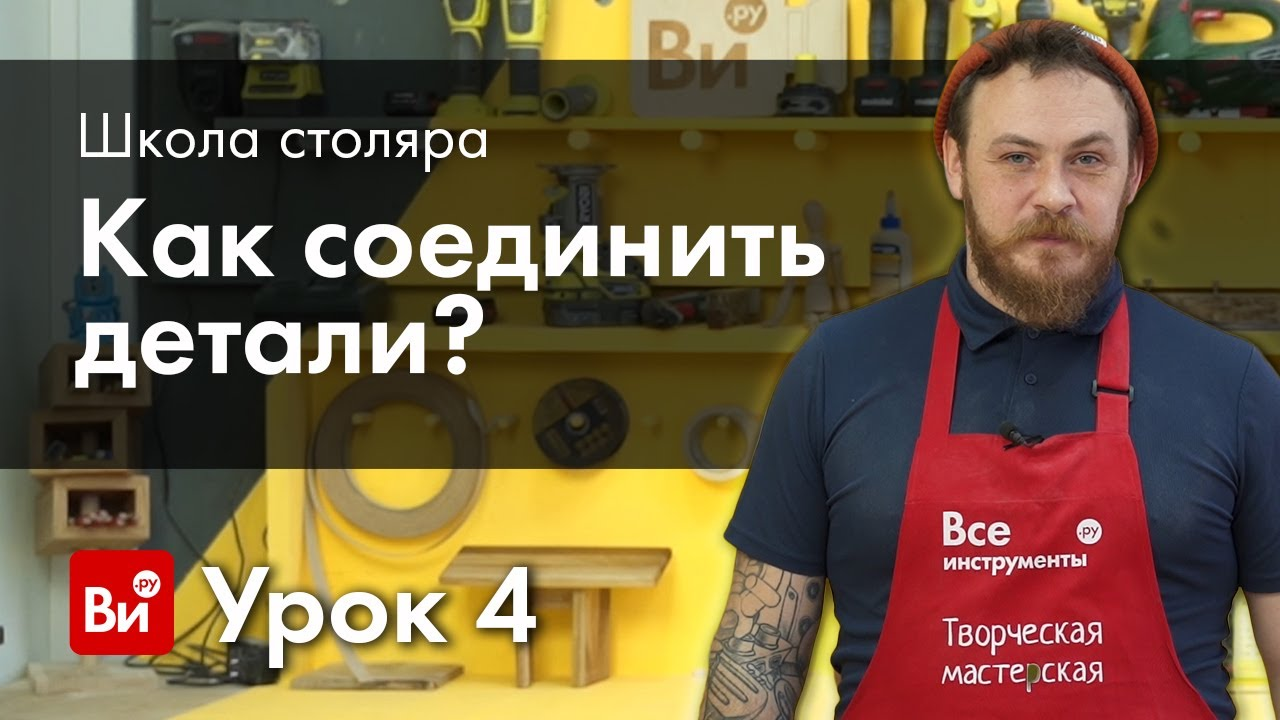
\includegraphics[height=6cm,width=1\textwidth,keepaspectratio]{glue_video.jpg}}
        \label{fig:glue_video.jpg}
    \end{figure}
\end{frame}

\begin{frame}[c]{Threadlocker (Фиксатор Резьбы)}
    \framesubtitle{}
    \vspace{-0.6cm}
    \begin{figure}[H]
        \centering\includegraphics[height=6cm,width=1\textwidth,keepaspectratio]{threadlocker.png}
        \label{fig:threadlocker.png}
    \end{figure}
\end{frame}

\begin{frame}[t]{Riveting (Заклепочное)}
    \framesubtitle{}
    \begin{columns}[T,onlytextwidth]
        \begin{column}{0.49\textwidth}
            The riveted joint is a permanent joint cause rivet is a permanent mechanical fastener. A rivet is a cylindrical shaft with a head on one end and the opposite end known as a tail.
            \medskip

            Used in structures, bridges, sheet metal operations, ships, and many industries. Main benefit --- \textbf{resistance to vibrations}.
        \end{column}
        \begin{column}{0.49\textwidth}
            \vspace{-1cm}
            \begin{figure}[H]
                \centering\includegraphics[height=6cm,width=1\textwidth,keepaspectratio]{rivetrivet.jpg}
                % \caption{caption_name}
                \label{fig:rivetrivet.jpg}
            \end{figure}
        \end{column}
    \end{columns}
\end{frame}

\begin{frame}[t]{Riveting in general}
    \framesubtitle{}
    \vspace{-0.6cm}
    \begin{figure}[H]
        \centering\includegraphics[height=6cm,width=1\textwidth,keepaspectratio]{rivets.png}
        \label{fig:rivets.png}
    \end{figure}
\end{frame}

\begin{frame}[t]{Rivets in aircrafting}
    \framesubtitle{Video}
    \vspace{-0.6cm}
    \begin{figure}[H]
        \href{https://youtu.be/IDbTUt3OG9s}{
            \centering\includegraphics[height=6cm,width=1\textwidth,keepaspectratio]{rivets_aircrafts_video.jpg}}
        \label{fig:rivets_aircrafts_video.jpg}
    \end{figure}
\end{frame}

\begin{frame}[t]{Rivets in leather industry}
    \framesubtitle{}
    \vspace{-0.6cm}
    \begin{figure}[H]
        \begin{subfigure}{0.32\textwidth}
            \centering\includegraphics[height=6cm,width=1\textwidth,keepaspectratio]{brigantine_top.jpg}
            % \caption{capture1}
            \label{fig:brigantine_top.jpg}
        \end{subfigure}
        \begin{subfigure}{0.32\textwidth}
            \centering\includegraphics[height=6cm,width=1\textwidth,keepaspectratio]{brigantine_hop.jpg}
            % \caption{capture2}
            \label{fig:brigantine_hop.jpg}
        \end{subfigure}
        \begin{subfigure}{0.32\textwidth}
            \centering\includegraphics[height=6cm,width=1\textwidth,keepaspectratio]{rivets_leather.jpg}
            % \caption{capture3}
            \label{fig:rivets_leather.jpg}
        \end{subfigure}
    \end{figure}
\end{frame}

\begin{frame}[t]{Riveting (RUS)}
    \framesubtitle{Video}
    \vspace{-0.6cm}
    \begin{figure}[H]
        \href{https://youtu.be/H7ssVv_MtNQ}{
            \centering\includegraphics[height=6cm,width=1\textwidth,keepaspectratio]{riveting_rus_video.jpg}}
        \label{fig:riveting_rus_video.jpg}
    \end{figure}
\end{frame}

\begin{frame}[t]{How to remove rivets}
    \framesubtitle{Video}
    \vspace{-0.6cm}
    \begin{figure}[H]
        \href{https://youtu.be/uG5plvIy3wk}{
            \centering\includegraphics[height=6cm,width=1\textwidth,keepaspectratio]{rivets_umount_video.jpg}}
        \label{fig:rivets_umount_video.jpg}
    \end{figure}
\end{frame}

\begin{frame}[t]{Riveting Rofl}
    \framesubtitle{Video}
    \vspace{-0.6cm}
    \begin{figure}[H]
        \href{https://youtu.be/mGOiPPM6pKM}{
            \centering\includegraphics[height=6cm,width=1\textwidth,keepaspectratio]{riveting_rofl_video.jpg}}
        \label{fig:riveting_rofl_video.jpg}
    \end{figure}
\end{frame}

\begin{frame}[t]{Riveting}
    \framesubtitle{Reference material}
    \begin{itemize}
        \item \href{https://www.theengineerspost.com/types-of-rivets/}{Types of rivets}
    \end{itemize}
\end{frame}



\begin{frame}[t]{Welding (Сварка)}
    \framesubtitle{}
    \begin{columns}[T,onlytextwidth]
        \begin{column}{0.49\textwidth}
            Welding is a fabrication process that joins materials, usually metals or thermoplastics, by using high heat to \textbf{melt the parts together} and allowing them to cool, causing fusion.
        \end{column}
        \begin{column}{0.49\textwidth}
            \begin{figure}[H]
                \centering\includegraphics[height=5cm,width=1\textwidth,keepaspectratio]{welding.jpg}
                \label{fig:welding.jpg}
            \end{figure}
        \end{column}
    \end{columns}
\end{frame}

\begin{frame}[t]{Difference between Welding and Soldering (Пайка) (RUS)}
    \framesubtitle{Video}
    \vspace{-0.6cm}
    \begin{figure}[H]
        \href{https://youtu.be/msRRSCB1G10}{
            \centering\includegraphics[height=6cm,width=1\textwidth,keepaspectratio]{diff_welding_soldering_video.jpg}}
        \label{fig:diff_welding_soldering_video.jpg}
    \end{figure}
\end{frame}

\begin{frame}[t]{Introduction to welding process}
    \framesubtitle{Video}
    \vspace{-0.6cm}
    \begin{figure}[H]
        \href{https://youtu.be/jQddm3YONNc}{
            \centering\includegraphics[height=6cm,width=1\textwidth,keepaspectratio]{into_to_welding_video.jpg}}
        \label{fig:into_to_welding_video.jpg}
    \end{figure}
\end{frame}

\begin{frame}[t]{Welding joint types}
    \framesubtitle{Video}
    \vspace{-0.6cm}
    \begin{figure}[H]
        \href{https://youtu.be/8kbUZLuhrW8}{
            \centering\includegraphics[height=6cm,width=1\textwidth,keepaspectratio]{weld_joint_types_video.jpg}}
        \label{fig:weld_joint_types_video.jpg}
    \end{figure}
\end{frame}

\begin{frame}[t]{Welding (RUS)}
    \framesubtitle{Video}
    \vspace{-0.6cm}
    \begin{figure}[H]
        \href{https://youtu.be/bCe_WB7vO-A}{
            \centering\includegraphics[height=6cm,width=1\textwidth,keepaspectratio]{welding_rus_video.jpg}}
        \label{fig:welding_rus_video.jpg}
    \end{figure}
\end{frame}

\begin{frame}[t]{Classical Welding techniques}
    \framesubtitle{Reference material}
    \begin{itemize}
        \item \href{https://www.youtube.com/watch?v=elmDvqdeMKI}{Stick (Ручная дуговая) (SMAW)}
        \item \href{https://youtu.be/twUAa5LWUvk}{MIG (С помощью Инертного газа) (GMAW)}
        \item \href{https://youtu.be/uO5pVLOAmD4}{TIG (Аргонодуговая)}
        \item \href{https://www.youtube.com/watch?v=TPSQJXqSwTg}{Flux Cored Arc (Порошковым флюсом)}
        \item \href{https://youtu.be/y-OKi8oSNQ4}{Another exlanation of all 4 types}
    \end{itemize}
\end{frame}


\begin{frame}[t]{Soldering (Пайка) \& Brazing (Высокотемпературная)}
    \framesubtitle{}
    \begin{columns}[T,onlytextwidth]
        \begin{column}{0.49\textwidth}
            It is a process in which two or more items are \textbf{joined by melting and putting a filler metal (solder) into the joint}, the \textbf{filler metal having a lower melting point} than the adjoining metal.
        \end{column}
        \begin{column}{0.49\textwidth}
            \begin{figure}[H]
                \centering\includegraphics[height=5cm,width=1\textwidth,keepaspectratio]{how_to_hold_solder.jpg}
                \label{fig:how_to_hold_solder.jpg}
            \end{figure}
        \end{column}
    \end{columns}
\end{frame}

\begin{frame}[t]{Difference between Soldering and Brazing}
    \framesubtitle{Video}
    \vspace{-0.6cm}
    \begin{figure}[H]
        \href{https://youtu.be/Rq_Vuye4HL0}{
            \centering\includegraphics[height=6cm,width=1\textwidth,keepaspectratio]{dif_sold_braz_video.jpg}}
        \label{fig:dif_sold_braz_video.jpg}
    \end{figure}
\end{frame}

\begin{frame}[t]{Soldering \& Brazing}
    \framesubtitle{Reference material}
    \begin{itemize}
        \item \href{https://www.uti.edu/blog/welding/brazing-soldering-welding}{Brazing soldering welding difference}
    \end{itemize}
\end{frame}

\begin{frame}[t]{Reference material}
    \framesubtitle{}
    \begin{enumerate}
        \item Mott R. L., Vavrek E. M., Wang J. Machine Elements in Mechanical Design, Ed. --- 2011
        \item Avallone E. A., Baumeister III T., Sadegh A. Marks' standard handbook for mechanical engineers. --- McGraw-Hill Education, 2007.
        \item Budynas R. G. et al. Shigley's mechanical engineering design. --- New York : McGraw-Hill, 2011.
        \item \href{https://youtu.be/jyun8hmWjS4}{Types of connection (rus, video)}
        \item \href{https://engineeringbookspdf.com/category/mechanical-engineering-pdf-books/}{A lot of engineering books in english}
    \end{enumerate}

    % 
\end{frame}



\fbckg{fibeamer/figs/last_page.png}
\frame[plain]{}

\end{document}